%% LyX 1.5.5 created this file.  For more info, see http://www.lyx.org/.
%% Do not edit unless you really know what you are doing.
\documentclass[a4paper,czech,czech,openright,cleardoubleempty,BCOR10mm,DIV11]{scrreprt}
\usepackage[T1]{fontenc}
\usepackage[utf8]{inputenc}
\usepackage{array}
\usepackage{longtable}
\usepackage{varioref}
\usepackage{wrapfig}
\usepackage{fancybox}
\usepackage{calc}
\usepackage{framed}
\usepackage{url}
\usepackage{graphicx}
\usepackage{placeins} %floatbarrier \FloatBarrier

\makeatletter

%%%%%%%%%%%%%%%%%%%%%%%%%%%%%% LyX specific LaTeX coěmmands.
\providecommand{\LyX}{L\kern-.1667em\lower.25em\hbox{Y}\kern-.125emX\@}
\newcommand{\lyxline}[1][1pt]{%
  \par\noindent%
  \rule[.5ex]{\linewidth}{#1}\par}
\newcommand{\noun}[1]{\textsc{#1}}
%% Special footnote code from the package 'stblftnt.sty'
%% Author: Robin Fairbairns -- Last revised Dec 13 1996
\let\SF@@footnote\footnote
\def\footnote{\ifx\protect\@typeset@protect
    \expandafter\SF@@footnote
  \else
    \expandafter\SF@gobble@opt
  \fi
}

\renewcommand{\baselinestretch}{1.2} %radkovani s

\expandafter\def\csname SF@gobble@opt \endcsname{\@ifnextchar[%]
  \SF@gobble@twobracket
  \@gobble
}
\edef\SF@gobble@opt{\noexpand\protect
  \expandafter\noexpand\csname SF@gobble@opt \endcsname}
\def\SF@gobble@twobracket[#1]#2{}
%% Because html converters don't know tabularnewline
\providecommand{\tabularnewline}{\\}

%%%%%%%%%%%%%%%%%%%%%%%%%%%%%% Textclass specific LaTeX commands.
\newenvironment{lyxcode}
{\begin{list}{}{
\setlength{\rightmargin}{\leftmargin}
\setlength{\listparindent}{0pt}% needed for AMS classes
\raggedright
\setlength{\itemsep}{0pt}
\setlength{\parsep}{0pt}
\normalfont\ttfamily}%
 \item[]}
{\end{list}}

%%%%%%%%%%%%%%%%%%%%%%%%%%%%%% User specified LaTeX commands.
%<-------------------------------společná nastavení------------------------------>
\usepackage[czech]{babel}%počeštění názvů (Obsah, Kapitola, Literatura atp.)
\usepackage[]{hyperref} %odkazy v  pdf jsou klikací s barevnými rámečky
\usepackage[numbers,sort&compress]{natbib} %balíček pro citace literatury  
\usepackage{hypernat}%interakce mezi hyperref a natbib
\newcommand{\BibTeX}{{\sc Bib}\TeX}%BibTeX logo
\hypersetup{   % Nastavení polí PDF dokumentu 
pdftitle={Platforma Vert.x},%   
pdfauthor={Michael Kutý},%  
pdfsubject={},%   
pdfkeywords={\v{s}ablona,LaTeX,LyX}%                             
}
\usepackage{multicol}




%<-----------------------------volání stylů----------------------------------------->
% (znak % je označení komentáře: co je za ním, není aktivní)
%<------------------------------------písmo----------------------------------------->
%\usepackage{packages/bc-latinmodern}
%\usepackage{packages/bc-times}
\usepackage{packages/bc-palatino}
%\usepackage{packages/bc-iwona}
%\usepackage{packages/bc-helvetika}


%<------------------------------záhlaví stránek------------------------------------>
%\usepackage{packages/bc-headings}
\usepackage{packages/bc-fancyhdr}

%<------------------------------hlavičky kapitol------------------------------------>
%\usepackage{packages/bc-neueskapitel}
%\usepackage{packages/bc-fancychap}

\makeatother

\usepackage{babel}

%java code block%

\usepackage{listings}
\usepackage{color}

\definecolor{dkgreen}{rgb}{0,0.6,0}
\definecolor{gray}{rgb}{0.5,0.5,0.5}
\definecolor{mauve}{rgb}{0.58,0,0.82}

% syntax highlight pro jazyk Java %
\lstset{
  %frame=r,
  language=Java,
  aboveskip=3mm,
  belowskip=3mm,
  xleftmargin=0.2mm,
  showstringspaces=false,
  columns=flexible,
  basicstyle={\small\ttfamily},
  numbers=none,
  numberstyle=\tiny\color{gray},
  keywordstyle=\color{blue},
  commentstyle=\color{dkgreen},
  stringstyle=\color{mauve},
  breaklines=true,
  breakatwhitespace=true,
  tabsize=3,
    inputencoding=utf8,
    extendedchars=true,
    literate=%
    {á}{{\'a}}1
    {č}{{\v{c}}}1
    {ď}{{\v{d}}}1
    {é}{{\'e}}1
    {ě}{{\v{e}}}1
    {í}{{\'i}}1
    {ň}{{\v{n}}}1
    {ó}{{\'o}}1
    {ř}{{\v{r}}}1
    {š}{{\v{s}}}1
    {ť}{{\v{t}}}1
    {ú}{{\'u}}1
    {ů}{{\r{u}}}1
    {ý}{{\'y}}1
    {ž}{{\v{z}}}1
    {Á}{{\'A}}1
    {Č}{{\v{C}}}1
    {Ď}{{\v{D}}}1
    {É}{{\'E}}1
    {Ě}{{\v{E}}}1
    {Í}{{\'I}}1
    {Ň}{{\v{N}}}1
    {Ó}{{\'O}}1
    {Ř}{{\v{R}}}1
    {Š}{{\v{S}}}1
    {Ť}{{\v{T}}}1
    {Ú}{{\'U}}1
    {Ů}{{\r{U}}}1
    {Ý}{{\'Y}}1
    {Ž}{{\v{Z}}}1
}

\begin{document}
%~\thispagestyle{empty}{\small ~\vfill{}
%}{\small \par}

%~\thispagestyle{empty}\vfill{}
%Tato stránka je tzv. protititul a je graficky součástí titulní stránky.
%Nechte ji prázdnou, nebo na ni umístěte vhodnou fotografii či ilustraci.

\cleardoublepage{}~\thispagestyle{empty}\begin{center}\pagenumbering{roman}\vspace{10mm}


\textsf{\textsc{\noun{\LARGE Univerzita Hradec Králové}}}\\
\vspace{0.5em}
\textsc{\noun{\LARGE Fakulta informatiky a managementu}}\\
\vspace*{1em}
\textsf{\textsc{\noun{\Large katedra informatiky a kvantitativních metod }}}

\vspace{15mm}


\includegraphics[width=0.4\textwidth]{logo/uhk}

\vspace{15mm}


\textsf{\huge BAKALÁŘSKÁ PRÁCE}{\huge \par}

\vspace{15mm}


\textsf{\LARGE Vert.x jako platforma pro webové aplikace}{\LARGE \par}

\vspace{10mm}


\end{center} 

\vspace*{\fill}


\vspace{10mm}


\begin{description}
\item [{{\large Autor:}}] \noindent \textsf{\large Michael Kutý}{\large \par}
\item [{{\large Vedoucí~práce:}}] \noindent \textsf{\large doc. Ing. Filip Malý, Ph.D.}{\large \hfill{}}\textsf{\large Hradec Králové, 2014}{\large{}
% doplňte rok vzniku vaší bakalářské práce
}{\large \par}
\end{description}
\clearpage{}

%{\small \thispagestyle{plain}\addcontentsline{toc}{chapter}{Abstrakt} }{\small \par}

\newpage{}\thispagestyle{plain}

{\small %\setcounter{page}{3} % nastavení číslování stránek
\ }{\small \par}

\noindent {\small \vfill{}
 % nastavuje dynamické umístění následujícího textu do spodní části stránky
~}{\small \par}

\subsubsection{Prohlášení}

\noindent {\small Prohlašuji, že jsem bakalářskou práci vypracoval samostatně a uvedl jsem všechny použité prameny a literaturu.}{\small \par}

{\small \bigskip{}
}\noindent {\small{} V Kroměříži dne \today\hspace{\fill}Michael Kutý}\\
{\small{} % doplňte patřičné datum, jméno a příjmení
}{\small \par}

\clearpage{}

\newpage{}\thispagestyle{plain}

{\small %\setcounter{page}{3} % nastavení číslování stránek
\ }{\small \par}

\noindent {\small \vfill{}
 % nastavuje dynamické umístění následujícího textu do spodní části stránky
~}{\small \par}

\subsubsection{Poděkování}

\noindent {\small Rád bych zde poděkoval doc. Ing. Filipu Malému, Ph.D. za odborné vedení práce, podnětné rady a čas, který mi věnoval. \newpage{}}{\small \par}

\clearpage{}

\newpage{}\thispagestyle{plain}

{\small %\setcounter{page}{3} % nastavení číslování stránek
\ }{\small \par}

\noindent {\small \vfill{}
 % nastavuje dynamické umístění následujícího textu do spodní části stránky
~}{\small \par}

\subsubsection{Anotace}

Bakalářská práce se zaměřuje na problematiku vývoje distribuovaných webových aplikací. Teoretická část práce popisuje architekturu platformy Vert.x a problémy, které tato platforma řeší. V praktické části bude implementovaná malá jednostránková kolaborativní aplikace jejíž jednotlivé části budou rozdistribuované na více instancí aby byla zajištěna vysoká dostupnost. Aplikace se nasadí do dvou referenčních instalací. První do prostředí VirtualBox a druhá v prostředí laboratoře CEPSOS při UHK.

\subsubsection{Annotation}

EN verze

\cleardoublepage{}

%\thispagestyle{empty}~{\small \addcontentsline{toc}{chapter}{Zadání
%práce} }{\small \par}



\newpage{}\thispagestyle{empty}~


{\small %%%   Výtisk pak na tomto míste nezapomeňte PODEPSAT!
%%%                                         *********
}{\small \par}

\cleardoublepage{}\thispagestyle{empty}{\small 
%\setcounter{secnumdepth}{3}
%\setcounter{tocdepth}{2}%hloubla obsahu
\tableofcontents{}% vkládá automaticky generovaný obsah dokumentu
\cleardoublepage{}}{\small \par}

\pagenumbering{arabic}%start arabic pagination from 1 


\chapter{Úvod}

V současné době existuje nespočet frameworků\footnote{jeho cílem je převzetí typických problémů dané oblasti, čímž se usnadní vývoj tak, aby se návrháři a vývojáři mohli soustředit pouze na své zadání}) pro vývoj webových aplikací ve spoustě programovacích jazycích. 
Výběr takového nástroje pak může být pro danou aplikaci klíčový. Vzhledem k faktu, že je s aplikací po celý životní cyklus, může se s časem stát svazujícím a nedostačujícím. Na reimplementaci však již není čas nebo peníze. Většina webových aplikací tak dříve nebo později narazí na na problematiku škálování, kdy je třeba rozložit aplikaci na více serverů ať už pro zajištění vysoké dostupnosti nebo kvůli velké výpočetní náročnosti. Dnes také není nic neobvyklého, že aplikaci najednou začnou navštěvovat tisíce klientů za minutu. Z dříve rychlé a stabilní aplikace se tak může stát často padající aplikace s nepřiměřenou odezvou.

Právě proto, jsem se rozhodl pro hlubší zkoumání v dané oblasti webových aplikací. V první části bakalářské práce popisuji architekturu a jednotlivé technologie, které mě motivovaly k hlubšímu studiu platformy Vert.x. V hlavní části práce následuje návrh, implementace a nasazení jednostránkové aplikace. V závěru je pak shrnutí kladů a záporů platformy.

\section{Cíl a metodika práce}

Hlavním cílem mé práce je zjištění zda-li se platforma Vert.x hodí pro vývoj distribuovaných webových aplikací. 
Vytvoření jednoduchého webového editoru pro správu myšlenkových map. %Jednostránkové webové aplikace pro kolaborativní práci s mindmapami. % 
Na této jednoduché aplikaci bude demonstrována architektura a nasazení aplikace na více serverů pro zajištění vysoké dostupnosti.
%proces vývoje a nasazení webové aplikace pod platformou Vert.x. Vzhledem k rozsahu práce budou popsány spíše principy a architektura daného řešení než implementační detaily. 
Zdrojové kódy včetně návodu na spuštění aplikace jsou umístěny veřejně na serveru Github\footnote{www.github.com/michaelkuty} a na přiloženém médiu.

Je nutné uchopit problematiku platformy Vert.x v širších souvislostech, proto se v práci snažím neopomenout všechny technologie, které s Vert.x souvisí, z kterých Vert.x vychází nebo které přímo integruje. V teoretické části bude čtenář seznámen s důležitými filozofiemi, které platforma nabízí. %A to jak událostmi řízenou architekturou, kterou platforma převzala z dnes již dobře známého frameworku Node.js\footnote{Serverový framework, postavený na modelu událostmi řízeného programování}. Tak především polyglot programování s jednoduchým konkurenčním modelem a možností sdílet data mezi jednotlivými vlákny bez nutnosti zámků.

Cílem teoretické části je tedy popsat jednotlivé architektonické prvky a komponenty platformy, jejich účel či problém, který řeší. V závěru teoretické části bude platforma srovnána s nástrojem Node.js. Srovnání bude obsahovat test výkonnosti a porovnání vlastností.

V praktické části bude vytvořen editor pro správu a tvorbu myšlenkových map. Tyto mapy bude moci spravovat více uživatelů najednou v reálném čase. Budou popsány a vysvětleny aspekty komunikace v reálném čase včetně samotného nasazení webové aplikace na jednotlivé servery, kde bude prověřena funkčnost distribuovaného provozu aplikace v režimu vysoké dostupnosti.

\section{Postup a předpoklady práce}

Práce předpokládá základní znalost programovacího jazyku Java a JavaScript. Teoretická část se neomezuje pouze na nezbytný popis technologií potřebných k realizaci malé jednostránkové webové aplikace. Představuje stručný pohled na celou platformu Vert.x. Teoretická část může být použita jako odraz k hlubšímu studiu daných technologií a konceptů. Praktická část bude prokládáná ukázkami kódu nebo příkazy souvisejícími s vývojem webových aplikací. Práce předpokládá znalost základní terminologie související s programováním obecně. Méně zažité pojmy budou vysvětleny poznámkou pod čarou.

Při vývoji webové aplikace budou použity následující softwarové technologie:
\begin{itemize}
\item Vert.x 2.1.2: platforma pro vývoj webových aplikací
\item MongoDB: dokumentově orientovaná NoSQL\footnote{databázový koncept, ve kterém datové úložiště i zpracování dat používají jiné prostředky než tabulková schémata tradiční relační databáze} databáze
\item D3.js: framework pro práci s grafy
\item JQuery framework pro práci s GUI(Graphical user interface)
\end{itemize}

%\pagenumbering{arabic}%start arabic pagination from 1 

\chapter{Platforma Vert.x}

Dnešním trendem internetu jsou real-time kolaborativní aplikace, které drasticky změnily potřeby programátorů, na jednotlivé nástroje. Programátor tak má možnost zvolit si z velké řádky nástrojů mezi než patří například Node.js, Akka či ruby EventMachine. Problémem těchto jinak časem a komunitou prověřených platforem může být fakt, že jsou úzce spjaté s konkretním programovacím jazykem či velmi náročná integrace do již stávájící aplikace.

Vert.x je projekt vycházející z Node.js, který jako první framework, pokořil v roce 2010 C10K\footnote{C10K problém řeší otázku: „Jak je možné obsloužit deset tisíc klientů za pomocí jednoho serveru, a to s co možná nejnižším zatížením serveru} problém. Obě platformy poskytují asynchronní API, které si je co do zaměření velice podobné. Node.js, jak již název napovídá je napsán v jazyce JavaScript, zatím co Vert.x je implementován v Javě. Vert.x ale není pouhá reimplementace Node.js do jazyka Java. Platforma má svou vlastní unikátní filozofii a terminologii, která je diametrálně odlišná od Node.js.

%Problém těchto jinak časem a komunitou ověřených platforem je fakt. Obě zmíněné platformy jsou napsány v dynamicky kompilovaném jazyku, což pro jádro stabilní aplikace přináší povinnost psát jak testy integrační, které testují funkčnost celého systému, tak i unit testy. 
%I když bude aplikace z větší části pokrytá testy, mohou se objevit problémy v podobě nečekaných pádů za běhu aplikace. To může být způsobeno například voláním neexistující metody či přiřazení proměnné do jiného typu než je ona sama. Toto bylo jedním z důvodů pro implementaci nového řešení v jazyce Java. Tento jazyk přináší platformě velkou stabilitu, rozšiřitelnost a zázemí v podobě tisícovek stabilních knihoven. Vert.x může být použit jako plnohodnotné řešení pro celou aplikaci nebo nasazen jako dílčí část architektury jiného řešení.

\section{Historie}

Začátek vývoje projektu Vert.x je datován do roku 2011. Tedy rok poté co spatřil světlo světa framework Node.js a za pouhý rok si vydobyl své místo u komunity, která si jej velmi oblíbila. Pravděpodobně největší motivací pro vývoj nové platformy podobné Node.js byla právě oblíbenost Node.js. 

Hlavním autorem platformy byl a je Tim Fox, který v době začátku vývoje platformy pracoval ve společnosti VMWare. Tato společnost si vzápětí nárokovala všechny zásluhy Tima Foxe na Vert.x platformu. Právníci společnosti vydaly výzvu, ve které požadovali mimo jiné doménu, veškerý zdrojový kód a účet Tima Foxe na Githubu. Z toho důvodu Tim Fox odešel od společnosti v roce 2012. V témže roce projevila o platformu zájem firma RedHat, která nabídla Timovi pracovní místo, absolutně volnou ruku ve vývoji a vedení projektu\citep{whoControlVertx}. 

Po několika debatách jak s představiteli společnosti RedHat tak i komunitou došel Tim Fox k názoru, že nejlepší pro budoucí zdravý rozvoj platformy bude přesunutí celé platformy pod nadaci Eclipse Foundation, k čemuž došlo na konci roku 2013. V dnešní době se platforma těší velkému vývoji, který čítá desítky  pravidelných přispěvatelů mezi něž patří mimo Tima například také Norman Maurer, který se řadí mezi přední inženýry vyvíjející framework Netty.io a zodpovídá za integraci Netty frameworku do platformy Vert.x.

Na tomto místě by bylo vhodné uvést, že platforma Vert.x letos vyhrála prestižní cenu "Most Innovative Java Technology" v soutěži JAX Innovation awards\citep{JAX}.

\section{Architektura}

Na obrázku \ref{fig:vertxArchitectureDiagram} jsou znázorněny dvě nezávislé Vert.x instance, které spolu komunikují pomocí zpráv. V levé části je blíže zobrazena jedna Vert.x instance, která bude blíže rozebrána v následujících kapitolách.

\begin{figure}
\begin{centering}
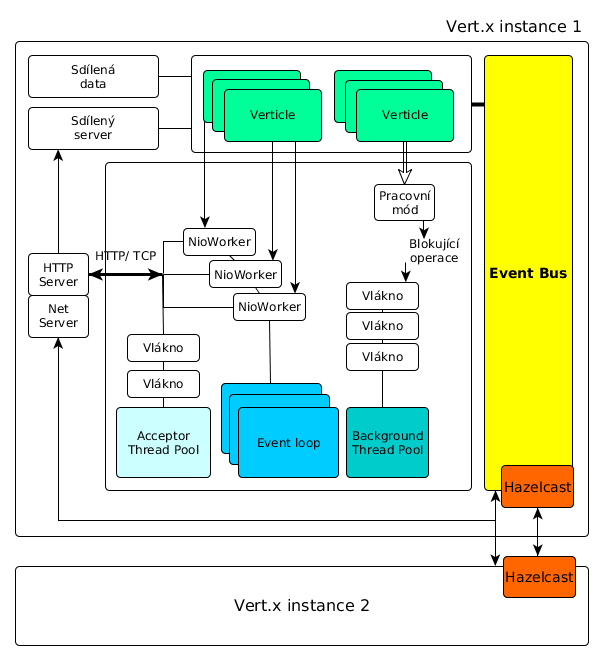
\includegraphics[scale=0.55]{obrazky/architecture_vertx}
\par\end{centering}
\caption{Architektura Vert.x převzato a upraveno z \cite{vertxArchitectureDiagram} \label{fig:vertxArchitectureDiagram}}
\end{figure}

\subsection{Jádro}

Velikost samotného jádra aplikace nepřekračuje 10Mb kódu v jazyce Java. V současné verzi je jádro platformy koherentní, dobře čitelné a poskytuje málé, ale za to stabilní API. Jak je popsáno v kapitole \ref{sub:API}, Vert.x se nesnaží umět vše, ale specializuje se na určitou činnost. 

Lze jej následně rozšířit o novou funkčnost dokompilovaním balíčků, které lze naleznout v oficiálním repositáři. Pravděpodobnou inspirací byl již zmíněný Node.js respektive NPM\footnote{Node package manager} u kterého se takováto forma vývoje velice oblíbila. Od doby vzniku této platformy vzniklo nespočet rozšíření, které udělaly z Node.js silný násroj pro rychlý vývoj webových aplikací. 
Klíčové jsou aspekty jako událostmi řízené programování a neblokující asynchronní model.

\noindent Zásadní technologie, které integruje Vert.x.
\begin{description}
\item[Netty.io] framework pro práci se vstupy a výstupy
\item[Hazelcast] In-memory data grid
\end{description}

Netty.io samotný, lze použít pro vývoj webových aplikací stejně dobře jako kterýkoliv jiný nástroj. Jeho specializací však je práce se vstupy a výstupy tzv. IO. V této oblasti poskytuje nízkoúrovňové API, nad kterým Vert.x přidává vyšší míru abstrakce. Druhou technologií, která je pro Vert.x klíčová je popsána v samostatné kapitole \ref{sub:hazelcast}.

\subsection{Asynchronní model}

Událostmi řízené programování je podle Tomáše Pitnera\cite{javaProgramovani} základním principem tvorby aplikací s GUI. Netýká se však pouze GUI, je to obecnější pojem označující typ asynchronního programování, kdy je tok programu řízen událostmi na které navěšuje tzv. event handlery\footnote{obslužná rutina události}.

Události nastávají obvykle určitou uživatelskou akcí(klik či pohyb myši, stisk tlačítka).
Událostmi řízené aplikace musí být většinou programovány jako vícevláknové (i když spouštění vláken obvykle explicitně programovat nemusíme).
Asynchronní někdy také paralelní model je přímo závislý na způsobu implementace samotným programovacím jazykem. Základním pojmem je zde proces, který je vnímán jako jedna instance programu, který je plánován pro nezávislé vykonávání. Naproti tomu Vlákno\footnote{Označuje v informatice odlehčený proces, pomocí něhož se snižuje režie operačního systému při změně kontextu, které je nutné pro zajištění multitaskingu} je posloupnost po sobě jdoucích událostí. V dřívější době nebylo potřeba rozlišovat proces a vlákno, protože proces se dále v aplikaci nedělil. Vytvoření vlákna je poměrně drahá a pomalá operace. Což se často obchází vytvořením zásoby uspaných vláken dopředu s nějakým managementem, co vlákna přidává a ubírá dle potřeby. Základním principem Vert.x a jemu podobných frameworků je jedno hlavní vlákno, obvykle pro každý procesor jedno. Takovéto vlákno si pak samo řídí vytváření a přidělování vláken.

Tento model bývá často kritizován, že nutí programátory psát špatně udržovatelný kód, především pak v situacích, kdy je potřeba koordinovat výsledky mezi více handlery. Pro tyhle situace ovšem vznikla řada nástrojů, které se liší podle použitého jazyka.

%respektive Node.js je tedy jedno hlavní vlákno, které si dle potřeby vytváří vlákna další a řídí tak . V jedné aplikace tedy může běžet několik vláken. Vlákno je zde bráno jako základní plánovací jednotka pro běh na procesoru. 
%Existují dva druhy asynchronního modelu (multitaskingu):
%multiprocesorový: o běh, tvorbu a režii vláken se stará operační systém
%multivláknový: o běh, tvorbu a režii vláken se stará aplikace a předává je operačnímu systému
%Podle Lažanského\cite{vlaknaCvut} je sdílení paměti důsledkem nižší režie při přepínání (přepnutí %vláken je výrazně rychlejší), obdobně i vytváření a rušení vlákna a samozřejmě i úspora paměti.
Samotné jádro Vert.x je implementováno v jazyce Java a pro Vert.x je tedy důležité, jak moc je dobrá implementace paralélního modelu v tomto jazyce. Neznamená to však, že se celá aplikace musí implementovat výhradně v jazyce Java. Jedinému požadavek pro běh Vert.x instancí je přítomnost Java development Kitu ve verzi 1.7 a novější. Tato verze přinesla nespočet vylepšení, pro jejichž výpis zde není místo. Došlo také na přepsání či úpravy v několika zásadních třídách z balíčku java.util.concurrent, což je třída zabývající se prací s multitaskingem a konkurencí.
\begin{description}
\item[ExecutorService]{z balíčku java.util.concurrent}
\item[CyclicBarrier\footnote{Synchronizační bariéra. Využitelná pro konstantní skupinu vláken, které mají přistupovat ke stejné proměnné. Třída zajištuje, že na sebe vlákna musí čekat při přístupu k proměnným. (Cyklická, protože jakmile se uvolní první vlákno jede to samé od znova)}]{z balíčku java.util.concurrent}
\item[CountDownLatch]{z balíčku java.util.concurrent}
\item[File]{z balíčku java.nio}
\item[Vylepšený ClassLoader\footnote{objekt zajištující načítání tříd}]{lepší odolnost vůči deadlockům\footnote{ je odborný výraz pro situaci, kdy úspěšné dokončení první akce je podmíněno předchozím dokončením druhé akce, přičemž druhá akce může být dokončena až po dokončení první akce.}}
\end{description}
\emph{Více o java.concurrent\cite{javaChangelog}}

Ed Gardoh v roce 2011 ve svém jednoduchém testu\cite{serialTest} prověřil práci s paralelizací úkonů. Z jeho testů vyplývá, že Java 1.7 je až o 40\% rychlejší při práci s vlákny nejenom díky nové metodě Fork/Join\cite{forkJoin}.

\subsubsection{Event loop}

Event Loops can be described as follows in a detailed way. Event Loops use Netty NioWorkder as it is. All handlers specified by verticles run on Event Loops. Each verticle instance has its specified NioWorker. As such, it is guaranteed that a verticle instance is always executed on an identical thread. Therefore, verticles can be written in a thread-safe manner.

Základem asynchronního modelu je vlákno, které se stará o všechny události. Když událost dorazí vlákno se postará o to aby byla zavolána ta správná obslužná rutina. Každá Vert.x instance interně obsluhuje malý počet těchto vláken, zpravidla pak jedno na každé procesorové jádro. Těmto vláknům se ve Vert.x komunitě říká \emph{Event Loop}. V komunitách Nginx nebo Node.js se ovšem setkáme spíše s pojmem \emph{Run Loop}. Přeloženo volně do češtiny pak ,,událostní smyčka". Obrovská nevýhoda takového přístupu je, že nikdy nesmí dojít k blokování takového vlákna. Jakmile k tomu dojde, celá aplikace tzv. zamrzne. Při startu verticlu \ref{sub:verticle} je pak vybrán jeden event loop, který ho obsluhuje po celý životní cyklus. Event loop je schopný obsloužit tisíce vertclů v ten samý čas.

Příklady blokujících volání:
\begin{itemize}
\item{tradiční API (JDBC, externí systémy)}
\item{dlouhotrvající operace (generování apod.)}
\end{itemize}

\subsubsection{Multi-reactor pattern}\label{sub:multireactor}

Základ jádra je postaven na tzv. Multi-reactor pattern\cite{eventLoops}, který vychází z Reactor patternu\cite{reactorPattern}, ten lze charakterizovat několika body:

\begin{itemize}
\item{aplikace je řízena událostmi}
\item{na události se registrují handlery}
\item{vlákno zpracovává události a spouští registrované handlery}
\item{toto vlákno nesmí být blokováno\footnote{pokud dojde k zablokování hlavního vlákna dojde k zablokování celé aplikace např.\emph{Thread.sleep(), a další z java.util.concurrent }}}
\end{itemize}

Multi-reactor pattern\cite{eventLoops} se od Reactor patternu liší pouze tím, že může mít více hlavních vláken. Tím přináší Vert.x možnost pohodlně škálovat instance na více procesorových jader. Jak je vidět z obrázku \vref{fig:instance} Vert.x platforma poskytuje více hlavních vláken, zpravidla však jedno hlavní vlákno na jeden procesor. Toho lze snadno docílit pomocí \emph{Runtime.getRuntime().availableProcessors()} o kterém se dozvíte více v kapitole \ref{sub:Scaling}. Na obrázku \vref{fig:instance4} pak lze vidět situaci čtyř hlavních vláken na čtyři procesorové jádra.

\subsubsection{Hybridní model vláken}\label{sub:hybrid}

Platforma Vert.x přišla s inovací v oblasti hlavních vláken a to takovou, že k hlavním \emph{Event loops} přidala další sadu vláken \emph{Background thread pool}, které jsou vyčleněny z hlavní architektury a poskytující samostatnou kapitolu pro škálování aplikace. To lze ostatně vidět na obrázku \vref{fig:vertxArchitectureDiagram}. Díky tomu, lze psát specializované moduly nebo verticle tzv. \emph{workery} pro blokující volání či dlouhotrvající operace aniž by nějak omezovaly běh celé aplikace. Více o \emph{workerech} v kapitole \ref{sub:moduly}.

\subsection{Terminologie}

Vert.x definuje svou vlastní terminologii, která je specifická jen pro tuhle platformu. Před dalším výkladem je tak nutné porozumět jednotlivým pojmům, které budou vysvětleny v následujících podkapitolách.

\subsubsection{Verticle}\label{sub:verticle}

Základní jednotka vývoje a nasazení. verticle si lze představit jako kus kódu v jazyce Java pak jako třídu s hlavní metodou. verticle je tak nejmenší funkční jednotkou Vert.x. verticle lze spouštět samostatně přímo z příkazové řádky podobně jako skript. Každý verticle běží ve vlastním vlákně z čehož plynou výhody, ale také nevýhody. Díky tomu, že každý verticle běží ve vlastním vlákně odpadá nutnost zámků nad proměnnýma, synchronizace vláken. V případě jedno vláknového modelu také odpadají deadlocky. Vzhledem k tomu, že každý verticle má svůj vlastní classloader nemůže tak sdílet statické metody ani hodnoty proměnných s ostatníma. Sdílet data je tak možné pouze dvěma způsoby.
\begin{itemize}
\item{pomocí Message Queue\cite{mq} dále jen MQ}
\item{SharedData object a SharedSet \emph{vertx.sharedData()}}
\end{itemize}
Objekty v SharedData musí být immutable\footnote{jakmile jednou takovýto objekt vznikne nejde dále měnit jeho proměnné}. V dnešní době je řada MQ frameworků přes které lze vést komunikaci u platformy Vert.x však není potřeba externí služba, protože má vlastní Event Bus o kterém pojednává kapitola \ref{sub:eventBus}. Na obrázku \ref{fig:instance} je vidět jeden verticle v kontextu jedné Vert.x instance. Následuje sumarizace vlastností verticle.

\begin{figure}
\begin{centering}
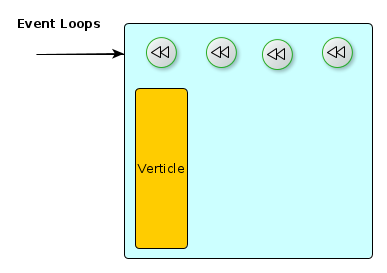
\includegraphics[scale=0.5]{obrazky/instance}
\par\end{centering}
\caption{Vert.x instance \label{fig:instance}}
\end{figure}

\begin{itemize}
\item nejmenší spustitelná jednotka
\item třída / skript
\item vykonává neblokující operace
\item běží vždy v jednom vlákně
\item přímý přístup k API, registrace handlerů, nasazení dalších verticlů
\end{itemize}

\subsubsection{Worker verticle}

V standardním verticlu by nemělo nikdy dojít k blokování hlavního vlákna. V dnešní době se bez klasického synchronního volání pravděpodobně neobejdeme, protože většina knihoven a modulů je napsána jako blokující kód. Z toho důvodu je v platformě Vert.x možnost označit verticle jako workera respektive pustit jej jako worker verticle metodou \emph{deployWorkerVerticle} namísto \emph{deployVerticle}. Tím dojde k vyčlenění verticle z asociace na hlavní vlákna a takovému vláknu pak bude přiděleno vlákno z Background thread poolu. Uvnitř takového verticle lze pak vykonávat blokující volání bez blokování celé aplikace. To v praxi nebývale rozšířilo možnosti uplatnění celé platformy. Bohužel tímto ztrácíme efektivní možnost škálování pro velký počet konkurenčních vláken je tedy vhodné situovat náročné výpočty na speciálně vyčleně servery. Velikost background thread poolu čítá na 20 před připravených vláken. Tento počet lze změnit v konfiguraci Vert.x.

\subsubsection{Vert.x instance}

Každý verticle běží uvnitř Vert.x instance \vref{fig:instance} a každá instance běží ve vlastní JVM instanci. V jedné Vert.x instanci může najednou běžet nespočet Vertclů. Všechny verticle můžou běžet souběžně na jednom serveru. Na jedno serveru může současně běžet mnoho Vert.x instancí v případě clusterování i na více serverech. verticle spolu pak komunikuji pomocí distribuovaného EventBusu.

\begin{figure}
\begin{centering}
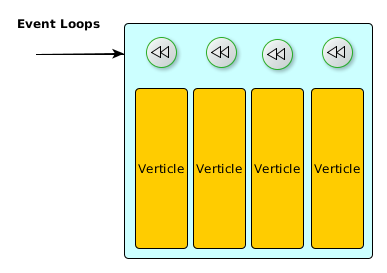
\includegraphics[scale=0.5]{obrazky/instance4}
\par\end{centering}
\caption{Příklad vertikálního škálování \emph{vertx run HelloWord -instances 4} \label{fig:instance4}}
\end{figure}

\subsubsection{Moduly}\label{sub:moduly}

Moduly poskytují možnost zapouzdření a znovupoužitelnost funkcionality. V praxi se mohou moduly skládat z více modulů či verticlů ve více programovacích jazycích. Modly mohou být uloženy v centrálním repozitáři\footnote{http://modulereg.vertx.io/} nebo může být využit jakýkoliv jiný repozitář. Repozitáře v kterých hledá Vert.x při startu instance dostupné moduly lze definovat v hlavní konfiguraci Vert.x. Každý modul musí mít svůj deskriptor ve formátu JSON\footnote{je odlehčený formát pro výměnu dat}. Jak může vypadat deskriptor je více popsáno v kapitole \ref{sec:praktickyModuly}.

Výhody plynoucí z použití modulů:
\begin{itemize}
\item{classpath\footnote{říká JVM, kde má hledat třídy a balíčky} je zapouzdřený a díky tomu lze moduly pouštět mnohem snáze}
\item{všechny závislosti jsou zapouzdřeny v jediném souboru ve formátu ZIP}
\item{moduly mohou být umístěny v repozitářích}
\item{Vert.x dokáže automaticky stahovat moduly, pokud je nenalezne v lokální instalaci}
\end{itemize}

Typy modulů lze rozdělit do dvou základních skupin, které lze dál rozdělit podle typu určení modulu.

\begin{description}
\item[spustitelné]{mají definovanou hlavní verticle v deskriptoru, takovéto moduly je pak možné spustit jako samostatné jednotky pomocí parametru \emph{runmod} nebo programově \emph{deployModule} }
\item[nespustitelné]{modul nemá specifikovaný hlavní verticle a lze jej použít v jiném modulu použitím metody \emph{includes}}
\end{description}

Pro vyčlenění modulu z asociace na event loop stačí přidat parametr \emph{worker: true} do deskriptoru modulu.

\subsection{Event Bus}\label{sub:eventBus}

Nervový systém celého Vert.x, jehož název lze volně přeložit jako sběrnice událostí. Cílem EventBusu je zpozdředkování komunikace mezi jednotlivými komponentami a vlákny aplikace. Podobně jako při použití externí MQ. Díky faktu, že komponenta Event Bus je implementována přímo v jádru platformy odpadá nutnost používat další knihovny pro práci s MQ a v neposlední řadě také režijní náklady či výpočetní výkon. Jak je vidět na obrázku , komponenta Event Bus je distribuovaná přes všechny instance v clusteru. Obrovskou výhodou oproti externí MQ je fakt, že lze takovouto komunikaci snadno přemostit ke klientovi na straně webového prohlížeče což je detailněji popsáno v kapitole \ref{sec:realTimeCommunication}.

\begin{figure}
\begin{centering}
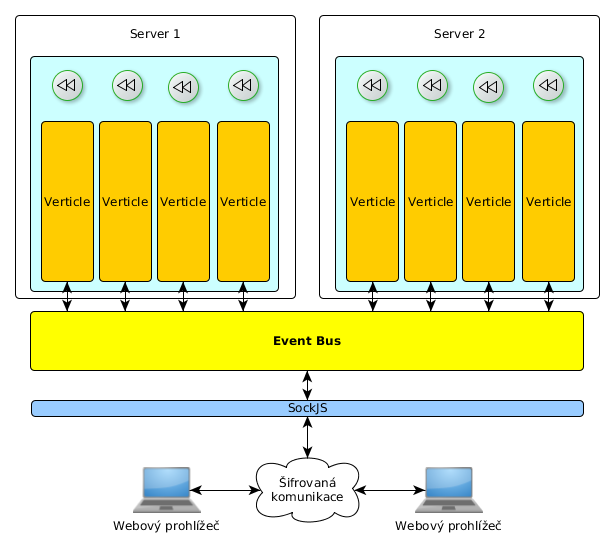
\includegraphics[scale=0.5]{obrazky/2instance4_eventbus}
\par\end{centering}
\caption{Event Bus distribuovaný mezi dva servery}
\label{fig:2instance4_eventbus}
\end{figure}

Základní typy komunikace:
\begin{itemize}
\item{Point to Point}
\item{Publish/Subscribe}
\end{itemize}

typy zpráv:
\begin{itemize}
\item{String}
\item{primitivní typy (int, long, short, float double, ..)}
\item{org.vertx.java.core.json.JsonObject}
\item{org.vertx.java.core.buffer.Buffer}
\end{itemize}

Toto je výčet pouze základních typů zpráv, které Vert.x podporuje v jádře. Není ale vůbec problém výčet stávájících typů rozšířit implementací vlastního modulu. Například modul bson.vertx.eventbus\footnote{https://github.com/pmlopes/mod-bson-io} rozšíří EventBus o možnost používat mnohem komplexnější typy zpráv jejichž výčet se nachází níže.

\begin{itemize}
\item{java.util.UUID}	
\item{java.util.List}
\item{java.util.Map}
\item{java.util.Date}
\item{java.util.regex.Pattern}
\item{java.sql.Timestamp}
\end{itemize}

Mezi doporučené se ovšem řadí JSON, protože je jednoduše serializovatelný mezi jednotlivými programovacími jazyky.

\subsubsection{Hazelcast}\label{sub:hazelcast}

Jednou z nejdůležitějších architektonických součástí Vert.x je knihovna Hazelcast, kterou tvoří jenom neuvěřitelných 3,1MB kódu v jazyce Java. V platformě Vert.x zaujímá důležité postavení jako In-memory data grid jehož vlastnosti \cite{inMemoryDataGrid} lze podle Ki Sun Song sumarizovat:
\begin{itemize}
\item{Data jsou distribuovaná a uložená na více serverech ve více geografických lokacích}
\item{Datový model je většinou objektově orientovaný a ne-relační}
\item{Každý server pracuje v aktivním režimu}
\item{Dle potřeby lze přidávat a odebírat servery}
\end{itemize}

Knihovnu Hazelcast lze využít v několika rolích:
\begin{itemize}
\item{NoSQL databáze v paměti}
\item{Cache\footnote{specializovaný typ paměti pro krátkodobé ukládání}}
\item{Data grid}
\item{Zasílání zpráv}
\item{Aplikační škálování}
\item{Clustrování aplikací}
\end{itemize}

Hazelcast je tedy typ distribuovaného úložiště, které běží jako vestavěný systém, lze díky němu distribuovat celou aplikaci a zasílat zprávy mezi jednotlivými komponentami. Vert.x API využívá Hazelcast API a odstiňuje tak programátora od poměrně nízko úrovňové API Hazelcastu.Když je Vert.x spuštěn, Hazelcast je spuštěn v módu vestavěného systému. Jako nejčastější příklad užití samotného Hazelcastu bývá uváděno ukládání uživatelské session\cite{session}. Hazelcast tedy usnadní práci v situaci, kdy budeme potřebovat uložit uživatelskou session například pro eshop. Mohli bychom využít externí RDBMS tedy databázový server, který by obstarával komunikaci s kleinty a udržoval integritu dat díky, kterému by jsme dosáhli stejného výsledku. S využitím knihovny Hazelcast ovšem odpadá nezbytná režie a monitoring, nemluvě o serverových prostředcích.

\section{API}\label{sub:API}

Vert.x poskytuje malou sadu metod, kterou lze volat na přímo z jednotlivých verticlů.
Funkcionalitu platformy lze jednoduše rozšířit pomocí modulů, které po zveřejnění do centrálního repozitáře může využívat kdokoliv a pomáhá tak znovu použitelnosti kódu. Samotné jádro Vert.x je tak velice malé a kompaktní. Vert.x API je rozděleno na \emph{Základní API} a \emph{Kontainer API}.

\subsection{Základní API}\label{sub:coreAPI}

Základní API, které Vert.x poskytuje programátorovi je poněkud strohé a obdobné jako u frameworku Node.js. Platforma tak poskytuje stabilní základ, který se v praxi neobejde bez modulů o kterých pojednává kapitola \ref{sub:moduly}.

\begin{itemize}
\item{TCP/SSL server/klient}
\item{HTTP/HTTPS server/klient}
\item{Websockets server/klient, SockJS}
\item{Distribuovaný Event Bus}
\item{Časovače}
\item{Práce s buffery}
\item{Přístup k souborovému systému}
\item{Přístup ke konfiguraci}
\end{itemize}

\subsection{Kontainer API}

Díky této části API může programátor řídit spouštění a vypínání nových modulů a verticlů za běhu aplikace. V praxi jsme tak schopní škálovat aplikaci za běhu či měnit funkcionalitu celé aplikace aniž by to někdo mohl zaregistrovat. Tuto API můžeme také volat přímo z příkazové řádky dále jen CLI\footnote{Command Line Interface}.

\begin{itemize}
\item{Nasazení a zrušení nasazení verticlů}
\item{Nasazení a zrušení nasazení Modulů}
\item{Získání konfigurace jednotlivých verticlů}
\item{Logování}
\end{itemize}

\subsection{Polyglot}

Polyglot je označován člověk, který ovládá více jazyků. V terminologii Vert.x to znamená, že API je dostupná ve více programovacích jazycích. Což v praxi znamená, že si programátor může sám zvolit v jakém jazyce bude implementovat svůj kód. Díky faktu, že spolu všechny verticly komunikují skrze zprávy je tak možné mít část aplikace napsanou například v jazyce Java a druhou část v jazyce Python apod. Tento fakt hodně napomáhá celé platformě nalákat nové programátory, protože ne každý, umí programovací jazyk Java. Výčet podporovaných jazyků ve verzi 2.0. Do verze 3.0 se pak chystá automatické generování API pro každý jazyk. 

\begin{itemize}
\item{Java}
\item{Javascript, CoffeeScript}
\item{Ruby}
\item{Python}
\item{Groovy}
\item{PHP}
\item{Clojure}
\end{itemize}

\section{Clustering}

Díky integraci Hazelcastu získala platforma Vert.x řadu zajímavých vlastností mezi které patří také možnost horizontálního škálování. Jak je vidět z obrázku \ref{fig:scaling_example}, jde o typ škálování do šířky, propojováním více serverových instancí dohromady. Na těchto instancích pak běží Vert.x platforma respektive Hazelcast, který spojuje všechny klienty dohromady. To v praxi znamená, že můžeme aplikace jednoduše škálovat přes více serverů bez nutnosti běhu dalších služeb a režijních nákladů. Přímo za běhu aplikace lze přidávat další Vert.x instance do clusterů. Samotná konfigurace clusteru není pak nic složitého a odehrává se v souboru \emph{conf/cluster.xml} a spočívá v nastavení členů clusteru nebo specifikování multicastové\footnote{logický identifikátor skupiny sítových hostů} adresy a portu na které bude Hazelcast po startu vyhledávat členy clusteru. Pro spuštění aplikace v režimu cluster ji stačí spustit s parametrem \emph{-cluster}. Pokud se na daném serveru nachází více síťových rozhraní je potřeba specifikovat \emph{-cluster-host}. Na tomto rozhraní pak bude komunikovat Hazelcast. V kapitole \ref{sub:praktCluster} je pak tato možnost využita pro běh Vert.x clusteru na odlišném rozhraní něž je běží webový server.
Velkou nevýhodou je pak nemožnost nasadit cluster na veřejné síti. V současné době Event Bus nepodporuje šifrované zprávy a jediná možnost jak toho dosáhnout, je pomocí nejrůznějších privátních tunelů. Ve verzi 3.0 má být plně implementována šifrovaná komunikace a nebude tak nic bránit nasazení na veřejné síti.
%Velkou výhodou je pak možnost šifrované komunikace, díky čemuž odpadá nutnost použití nejrůznějších služeb zajištující šifrování komunikace na sítové vrstvě v případě nasazení na veřejné síti nebo ve více geografických lokacích. 

\begin{figure}
\begin{centering}
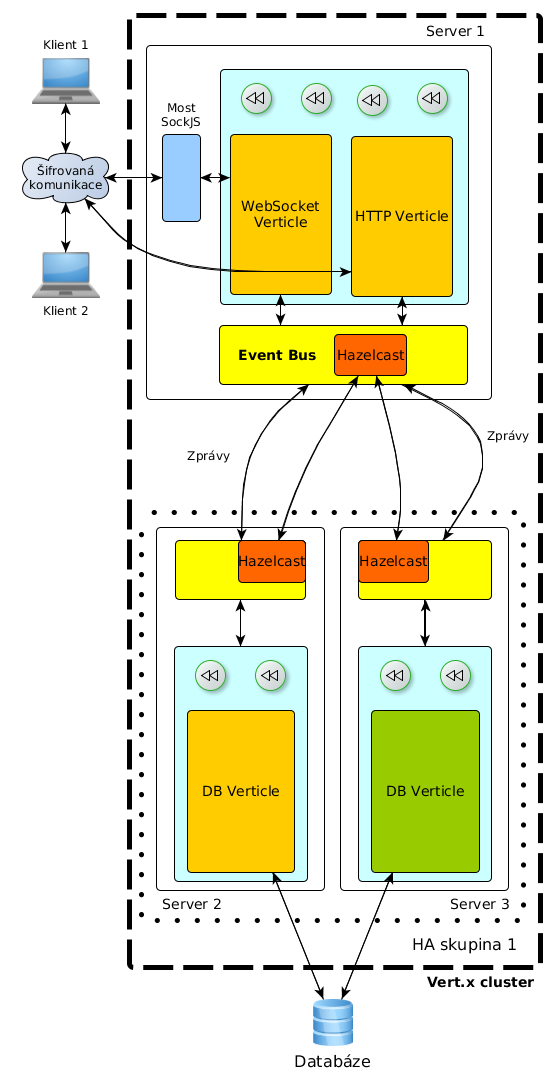
\includegraphics[scale=0.5]{obrazky/instance4_eventbus_geolocation}
\par\end{centering}
\caption{Clustering mezi třemi Vert.x instancemi \label{fig:instance4_eventbus_geolocation}}
\end{figure}

\subsection{Vysoká dostupnost}

Samostatnou kapitolou v oblasti clusteringu je HA\footnote{HA - High Availability} česky tedy vysoká dostupnost. Díky Hazelcastu ji lze řešit již na aplikační úrovni, a není potřeba  dalších služeb, které řeší vysokou dostupnost.

\subsubsection{Automatické zotavení z havárie}

Pokud je modul spuštěn s argumentem \emph{-ha} a dojde k pádu Vert.x instance. Modul bude automaticky nasazen na jiné instanci v clusteru. V takovém případě již není potřeba spouštět modul s parametrem \emph{-cluster}. Jak je vidět na obrázku \ref{fig:instance4_eventbus_geolocation} v případě pádu Serveru 2, tedy části aplikace, která komunikuje s databází dojde automaticky k novému nasazení této části do nové instance, která je taky členem Vert.x clusteru. Výpadek tak bude pro uživatele skoro nepostřehnutelný.

\subsubsection{Skupiny HA}

V případě spuštění modulů v režimu HA lze pak specifikovat logické skupiny. Pro spuštění instance v určité HA skupině stačí přidat parametr \emph{-hagroup <jméno skupiny>}. Díky tomu lze přesně určit, kde se mají moduly v případě pádu nasadit. To je v praxi vhodné především v situacích, kdy je do internetu vystavena pouze část clusteru. Například jako na obrázku \ref{fig:architecture_ideal}.

\subsubsection{Kvorum}

Při spuštění Vert.x instance lze specifikovat kvorum\footnote{minimální počet serverů pro zajištění vysoké dostupnosti}. Pokud nebude splněno kvorum nebude instance nasazena v režimu HA. Kvorum lze pak snadno spočítat ze vzorce \emph{Q = 1 + N/2}, kde N je počet serverů. Pokud dojde při běhu aplikace k porušení kvora bude režim HA automaticky vysazen.

\section{Porovnání s Node.js}

V následující kapitole bude porovnána platforma Vert.x s již zmíněnou platformou Node.js. Výkonnostní test\cite{benchmarkTim} je převzat od samotného autora projektu a jsou v něm zahrnuty jazyky, které v té době platforma podporovala. V druhé části kapitoly \ref{sub:performence} je pak tabulka\ref{table:odezvy} srovnání odezev s vybranými webovými platformami z daty ze zdroje\cite{benchmark}.

\subsection{Výkon}\label{sub:performence}

Tato kapitola se zabývá výkonnostními testy jednotlivých platforem. V prvním testu je obsaženo více programovacích jazyků, ve kterých byla implementována stejná logika pod platformou Vert.x. Rychlost aplikace implementované v jiném jazyce než Javě je pak závislá na konkrétním adaptéru.

\subsubsection{Metody testování}

V obou testech je testovaná aplikace škálovaná na šest procesorových jader tedy byla spuštěna s parametrem \emph{-instances 6}, oproti tomu je spuštěna aplikace Node.js ve dvou variantách. Samostatná a šest procesů v jednom clusteru. V legendě grafů je to odlišeno příponou \emph{cl}.

\begin{enumerate}
\item{Triviální dotazování serveru a návrat statusu 200\footnote{HTTP status - OK}}
\item{Dotaz na statický soubor o velikosti 72 bytů}
\end{enumerate}

\subsubsection{Hardware}

V prvním testu od Tima Foxe je požit  AMD Phenom II X6, 8GB RAM a systém Ubuntu 11.04. Tento procesor se 6 jádry není úplně běžný proto je výklad doplněn o druhý test, který proběhl na Sandy Bridge Core i7-2600K, 8GB RAM a SSD disku a systému Ubuntu 12.04.

\subsubsection{Výsledky}

Jak lze vidět na obrázku \ref{fig:test1} a \ref{fig:test2} výsledky obou testů lze shrnout do jedné věty. Vert.x zvládá řádově o desítky tisíc více odpovědí než platforma Node.js a i v případě režimu clusteru.

\begin{figure}
\begin{centering}
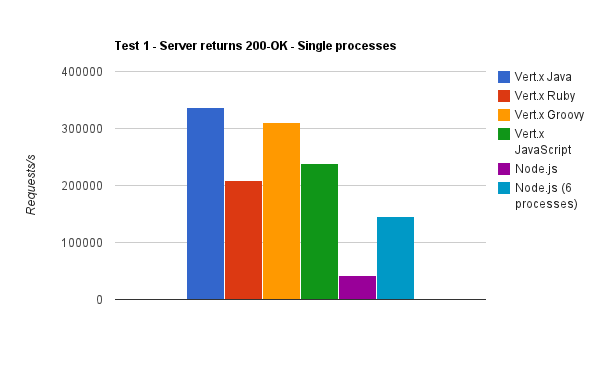
\includegraphics[scale=0.7]{obrazky/chart_1}
\par\end{centering}
\caption{Výsledky prvního testu \emph{Tim Fox} \cite{benchmarkTim}\label{fig:test1}}
\end{figure}

\begin{figure}
\begin{centering}
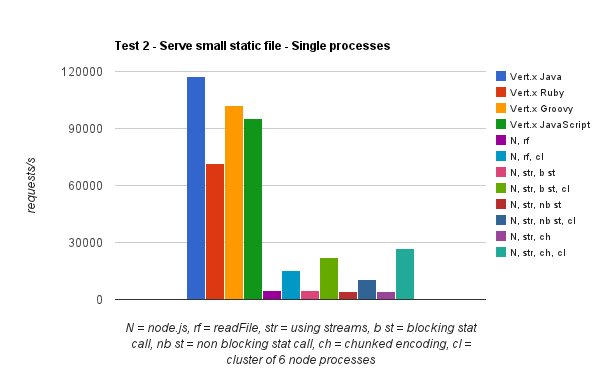
\includegraphics[scale=0.7]{obrazky/chart_3-5}
\par\end{centering}
\caption{Výsledek druhého testu \emph{Tim Fox} \cite{benchmarkTim}\label{fig:test2}}
\end{figure}

\subsubsection{Srovnání s vybranými platformami}

Metoda srovnání s ostatními platformami je založená na podobném principu jako předchozí testy s tím rozdílem, že místo statického souboru vrací odpověď ve formátu JSON. Na straně serveru tedy musí dojít k JSON serializaci.

\begin{flushleft}
\begin{longtable}{|c|c|c|}
\hline
\textsf{\textbf{Platforma}} & \textsf{\textbf{Průměrná odezva}} & \textsf{\textbf{Maximální}}\tabularnewline
\hline
Vert.x & 1,2ms & 18,7ms\tabularnewline
\hline 
Netty & 1,3ms & 24,0ms\tabularnewline
\hline
Ruby on Rails & 1.8ms & 241.6\tabularnewline
\hline 
Node.js & 3.7ms & 12,5\tabularnewline
\hline 

\caption{Srovnání odezvy, \emph{převzato a upraveno z} \cite{benchmark}}
\label{table:odezvy}
\end{longtable}
\end{flushleft}

\subsection{Vlastnosti}

Následující tabulka ukazuje srovnání důležitých vlastností jednotlivých platforem, jejichž důležitost byla popsána v předchozích kapitolách.

\begin{flushleft}
\begin{longtable}{|c|c|c|}
\hline
\textsf{\textbf{Vlastnost}} & \textsf{\textbf{Node.js}} & \textsf{\textbf{Vert.x}}\tabularnewline
\hline
CLI & Ano & Ano\tabularnewline
\hline 
Cluster & Ano & Ano\tabularnewline
\hline
Moduly & Ano & Ano\tabularnewline
\hline 
HA & Ne & Ano\tabularnewline
\hline
MQ & Ne & Ano\tabularnewline
\hline 
Hybridní model vláken & Ne & Ano\tabularnewline
\hline 
In-memory data grid & Ne & Ano\tabularnewline
\hline 
Polygnot & Ne & Ano\tabularnewline
\hline
\caption{Srovnání vlastností s Node.js}
\end{longtable}
\par\end{flushleft}

\subsection{Závěr srovnání}

Výsledkem srovnání je tedy fakt, že pokud by se dnes někdo rozhodoval o výběru platformy pro novou real-time aplikaci měl by určitě zvolit platformu Vert.x, která poskytuje řádově větší výkon a počet vlastností, nehledě na fakt, že v případě Node.js lze psát aplikaci pouze v jazyce JavaScipt, který se může jevit jako naprosto nevhodný pro Enteprise aplikaci.

%\pagenumbering{arabic}%start arabic pagination from 1 

\chapter{Praktická část}

V této kapitole je popsán software a postupy použité při implementaci a distribuovaném nasazení malé Vert.x aplikace pro správu myšlenkových map.

\section{Návrh}

Aplikace bude složena ze dvou částí. Serverová část, která bude pracovat s mapami a databází. Druhá část bude obsluhovat klienty na straně webového prohlížeče, tedy část realizovaná pomocí D3.js, která bude mít na starosti vykreslování a obsluhu iniciovaných akcí.	Obě části budou realizovány převážně v jazyce JavaScript, který s kterým každý programátor přišel určitě do styku.

\subsection{Cíle aplikace}\label{sub:use_case}

\begin{figure}[h]
\begin{centering}
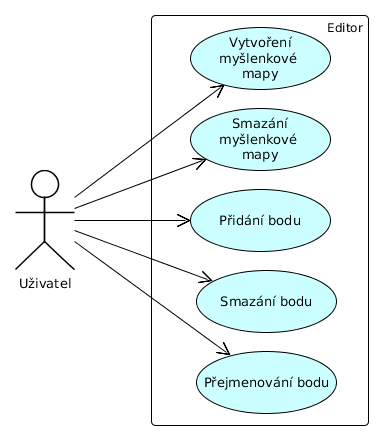
\includegraphics[scale=0.5]{obrazky/use_case}
\par\end{centering}
\caption{Případy užití\label{fig:use_case}}
\end{figure}

Hlavní cíle aplikace jsou:
\begin{itemize}
\item Přidání a odstranění myšlenkové mapy
\item Přidání a odstranění bodu v myšlenkové mapě
\item Přejmenování bodu v myšlenkové mapě
\end{itemize}

%\FloatBarrier

\subsection{Architektura}

Jak je vidět na obrázku \ref{fig:architecture_real}, klienti se budou připojovat přes jeden webový server, který bude mít otevřený port 80. S druhým serverem bude spojený na úrovni Hazelcast clusteru. Vzhledem k situaci, která je blíže popsaná v kapitole \ref{sub:praktCluster}, kdy je webový server připojen do dvou sítí není potřeba šifrování ani nejrůznějších tunelů. Druhý server bude sloužit pro komunikaci s databází a také jako \emph{exporter} myšlenkových map do obrázků ve formátu PNG. Modul \emph{exporter} bude implementován v jazyce Java jako demonstrace polyglot vývoje.

\begin{figure}[h]
\begin{centering}
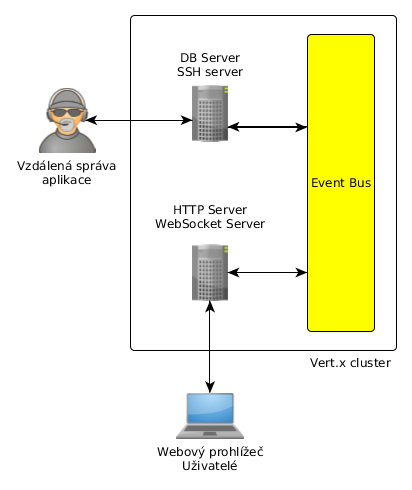
\includegraphics[scale=0.5]{obrazky/architecture_real}
\par\end{centering}
\caption{Architektura nasazené aplikace\label{fig:architecture_real}}
\end{figure}

%\FloatBarrier

\section{Komunikace v reálném čase}\label{sec:realTimeCommunication}

Po načtení myšlenkové mapy přichází na řadu aspekty komunikace v reálném čase. V rámci editoru myšlenkových map budou implementovány tři základní operace.
\begin{itemize}
\item Přidání objektu do myšlenkové mapy
\item Odstranění objektu z myšlenkové mapy
\item Přejmenování objektu v myšlenkové mapě
\end{itemize}

\begin{figure}[h]
\begin{centering}
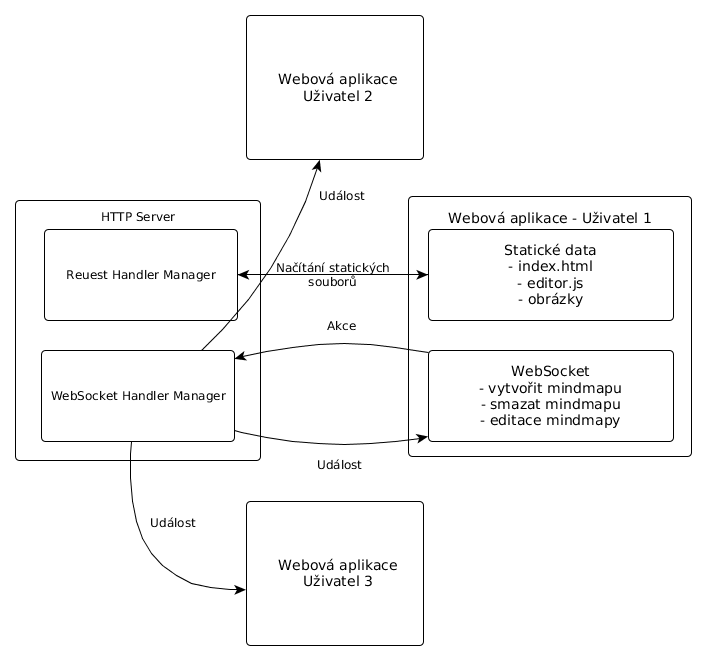
\includegraphics[width	=1\textwidth]{obrazky/realtime_communication}
\par\end{centering}
\caption{Komunikace v reálném čase\label{fig:realtime_communication}}
\end{figure}

V tradiční webové aplikaci by to znamenalo implementaci těchto metod typem požadavek-odpověď jako operací konkrétní API. Při přidání objektu by se zavolala API a nazpět by přišla odpověď, zda-li byla akce úspěšná. Pokud bychom však chtěli mít editor, který by propagoval změny ke všem, kdo mají myšlenkovou mapu otevřenou museli bychom znát přihlášené uživatele, kterým by server poslal notifikaci o změně. Mnohem jednoduší cesta je rozdělení požadavku a odpovědi do dvou částí což odpovídá návrhovému vzoru Command. V takovém případě při otevření webového prohlížeče s danou myšlenkovou mapou dojde k zaregistrování klienta na určitou adresu. V případě jakékoli změny, kterou provede jiný uživatel nebo kdokoliv jiný, dojde k odeslání události všem zaregistrovaným klientům okamžitě v době vykonání události. Tuto situaci lze vidět na obrázku \ref{fig:realtime_communication}. V případě, kdy u uživatele dojde k vyvolání akce, ostatním uživatelům bude zaslána událost, která s sebou nese všechny informace o změně. Všem klientům zaregistrovaným na stejnou adresu přijde stejná událost. Tento typ zasílání zpráv je znám jako návrhový vzor Publish/Subscribe.

\subsection{Akce}

Když bude uživatel chtít změnit myšlenkovou mapu (přidat objekt, odebrat objekt nebo přejmenovat objekt), vyšle akci na server. Tato akce bude poslána přes přemostěný event bus, které jsem představil v kapitole \ref{sub:eventBus}. Na straně serveru je pak verticle, který má zaregistrovány metody na příchozí akce. Samotná akce nemá žádnou návratovou hodnotu, pokud tak dojde k chybě nedojde k vyslání události, která s sebou nese změny myšlenkové mapy.

\subsection{Události}

Pokud uživatel otevře webový prohlížeč s konkrétní myšlenkovou mapou, dojde tak k přihlášení odběru událostí nad touto myšlenkovou mapou. Pokud ji někdo změní tento uživatel dostane stejnou událost s informací o změně jako každý jiný uživatel přihlášený k odběru událostí.
Na straně klienta tak budou implementovány metody, které budou mít definované chování pro každou z definovaných událostí: přidání, odebrání a přejmenování objektu v myšlenkové mapě.

\subsection{Klientská aplikace}

V následující kapitole jsou objasněny technologie použité na straně webového prohlížeče.


\section{Vlastní implementace}

Vzhledem k rozsahu práce je v následující kapitole ukázán a popsána většina implementačních částí.

\subsection{Řídící verticle}

Nasazení aplikace na více serverů s sebou přináší malé rozhodnutí. Jestli aplikaci rozdělíme do více menších modulů nebo jednu větší pustíme na více serverech ve více rolích. S přihlédnutím na rozsah aplikace je výhodnější implementovat řídící verticle, který bude mít na starost nasazovat moduly, dle dané konfigurace. Část kódu takového startéru vypadá následovně:

\begin{lstlisting}[caption=Řídící verticle]
var container = require('vertx/container');
var console = require('vertx/console');

var config = container.config;

if("webserver" in config) {
	container.deployModule('io.vertx~mod-web-server~2.0.0-final', config.webserver, config.webserver.workers, function(err, ID){
		if (err) {
			console.log(err)
		}
	});
}
\end{lstlisting}

Každá metoda \emph{deploy} má jako poslední parametr obslužnou rutinu pro případ selhání. V mnoha případech se také hodí ID nasazení, díky němuž lze později toto nasazení zrušit.

Samotný kód vytáhne z třídy \emph{container} konfiguraci celého modulu a zeptá se jestli se v něm nenachází daná role. Potom už jen stačí, aby daný konfigurační soubor obsahoval klíč \emph{webserver} s danou konfigurací, která se nachází níže. Obdobně je implementováno startování editoru, databázového modulu a exportéru. Spuštění modulu či verticle jde samozřejmě i ručně z příkazové řádky.

\begin{lstlisting}[caption=Spuštění modulu z příkazové řádky]
vertx runmod io.majklk~mindmapeditor~0.0.1 -conf /srv/mindmap/conf/webserver.json -instances 3
\end{lstlisting}

Spuštěním modulu z příkazového řádku se Vert.x podívá do deskriptoru modulu, v kterém by měl najít cestu k hlavnímu verticlu. Ten následně spustí a předá mu danou konfiguraci. Samotný verticle pak může pracovat s Vert.x instancí.

\begin{lstlisting}[caption=Konfigurace serveru 1]
{
   "name": "MindMap editor server 1 - HTTP + WebSocket",
    "webserver": {
        "workers": 3,
        "web_root": "web",
        "host": "10.10.10.161",
        "port": 80,
        "bridge": true,
        "inbound_permitted": [
          { "address": "mindMaps.list" },
          { "address": "mindMaps.save" },
          { "address": "mindMaps.delete"},
          { "address": "mindMaps.exporter.svg2png" },
          { "address_re": "mindMaps\\.editor\\..+" }
        ],
        "outbound_permitted": [
          { "address_re": "mindMaps\\.events\\..+" }
        ]
    }
}
\end{lstlisting}

Většina jmen parametrů mluví sami za sebe, kromě \emph{bridge, inbound permitted a outbound permitted}. Pokud je první z nich nastaven na hodnotu \emph{true}, tak začnou platit pravidla, která jsou nadefinována v \emph{inbound permitted, outbound permitted}. Jde o tzv. bridge mezi webovým prohlížečem a Event busem jako takovým. \emph{Inbound permitted} říká jaké adresy se mají pustit dovnitř, analogicky potom \emph{outbound permitted} říká, co může jít ven. Výhodou je pak možnost specifikovat adresu pomocí regulárních výrazů.

\subsubsection{Základní adresářová struktura}

\begin{lstlisting}
main.js //stará se o spouštění celé aplikace v několika rolích
editor.js //obsluha editoru
database.js //obsluha událostí 
web //kořenová složka webové části
\end{lstlisting}

\subsection{Editor}

\begin{lstlisting}[caption=Zaregistrování obslužné rutiny v jazyce JavaScript]
var eb = vertx.eventBus;

var mujHandler = function(zprava) {
  console.log('Přišla zpráva ' + zprava);
}

eb.registerHandler('test.tisk', mujHandler);
\end{lstlisting}

Obdobně to pak vypadá v ostatních jazycích. 

\begin{lstlisting}[caption=Zaregistrování obslužné rutiny v jazyce Java]
EventBus eb = vertx.eventBus();

Handler<Message> mujHandler = new Handler<Message>() {
    public void handle(Message zprava) {
        System.out.println("Přišla zpráva " + zprava.body);
    }
};

eb.registerHandler("test.tisk", mujHandler);
\end{lstlisting}

Na podobném principu je pak postaven zbytek serverové části. Na jednotlivé události jsou zaregistrovány podobné obslužné rutiny, které většinou dohledají konkrétní mapu a provedou nad ní nějakou změnu. Výslednou mapu uloží a pošlou událost všem klientům jako je vidět na diagramu \ref{fig:realtime_communication}.

\begin{lstlisting}[caption=Publikování zprávy v jazyce JavaScript]
eventBus.publish('editor.udalosti.'+mindMap._id, {"udalost": "bodPridan", parentKey: args.parentKey, node: newNode})
\end{lstlisting}

Díky metodě \emph{publish}, která je samozřejmě dostupná ve všech jazycích můžeme publikovat událost všem klientům, kteří mají zaregistrovanou obslužnou rutinu na identickou adresu, která je unikátní pro každou mapu.

\vspace{0.5cm} % fix

\subsection{Integrace s databází MongoDB}

Vzhledem k jednoduchosti aplikace nebyl vytvořen diagram tříd. V aplikaci budou pouze dva modely, a to mapa a její potomek, který se od mapy liší pouze tím, že má místo globálního unikátního identifikátoru pouze unikátní identifikátor v rámci jedné mapy.

V centrálním repozitáři již existuje modul pro komunikaci s MongoDB\footnote{https://github.com/vert-x/mod-mongo-persistor}, který poskytuje jednoduchou API pro asynchronní komunikaci s databází. Zaregistrujeme tedy obslužnou rutinu pro uložení myšlenkové mapy. Obdobně pak pro každou akci z definovaných cílů.

\begin{lstlisting}[caption=Uložení myšlenkové mapy do databáze]
var eventBus = require('vertx/event_bus');
var console = require('vertx/console');

eventBus.registerHandler('mindMaps.save', function(mindMap) {
	dotaz_do_databaze = {action: "save", collection: "mindMaps", document: mindMap}
	eventBus.send('vertx.mongopersistor', dotaz_do_databaze, function(reply) {
		if (reply.status === "ok") {
			// vše v pořádku
		} else {
			console.log(reply.message);
		}
	});
});

\end{lstlisting}

\begin{lstlisting}[caption={Konfigurace serveru 2},label=confServ2]
{
    "name": "MindMap editor server 2 databázový modul, obrazkový exporter",
    "exporter": {
        "workers": 5
    },
    "mongodb": {
        "address": "vertx.mongopersistor",
        "host": "localhost",
        "port": 27017,
        "db_name": "mindmap_editor",
        "pool_size": 20
    },
    "shell": {
      "crash.auth": "simple",
      "crash.auth.simple.username": "admin",
      "crash.auth.simple.password": "heslo",
      "crash.ssh.port": 2000
    }
}
\end{lstlisting}

\begin{description}
\item[\_id] unikátní identifikátor\footnote{podtržítkem se běžně označující neměnné proměnné}
\item[name] název samotné mapy
\item[children] potomci
\end{description}

\begin{lstlisting}
\end{lstlisting}

\begin{lstlisting}
{
	"_id": "1234-6545-5612-3456",
	"name": "Živočichové",
	"children": [
		{
			"key": "1",
			"name": "Obratolvci",
			"children": [
				{
					"key": "2",
					"name": "Ryby"
				},
				{
					"key": "3",
					"name": "Plazi"
				}
			]
		},
		{
			"key": "4",
			"name": "Bezobratlí"
		}
	]
}
\end{lstlisting}

\subsubsection{Struktura webové části}

\begin{lstlisting}
index.html
js/client.js //obsluha editoru
js/editor.js //vykreslování grafu - D3.js
js/vertxbus.js //knihovna pro napojení na Event Bus
css //složka pro kaskádové styly
\end{lstlisting}


\subsubsection{Event Bus v prohlížeči}

Nejdůležitější částí klientské aplikace je Vert.x vrstva nad SockJS\cite{sockjs}, která zabaluje komunikaci se serverem na protokolu WebSocket\cite{webSockets}. Knihovna naváže a udržuje neustálé spojení se serverem. Implementací metod \emph{eb.onopen a eb.onclose} může patřičně reagovat na otevření a uzavření spojení. Jediným parametrem samotného EventBusu je pak URL adresa na kterou se má připojit.

\begin{lstlisting}[caption=Připojení Event busu z prohlížeče a inicializace editoru]
var eb = new vertx.EventBus(window.location.protocol + '//' + window.location.hostname + ':' + window.location.port + '/eventbus');

eb.onopen = function() {
	//tato metoda se volá po úspěšném navázání komunikace
	//zde již můžeme posílat zprávy
	eb.send("mindMaps.save", mapa, function(reply){
		eb.send("mindMaps.find", mapa._id, function(mindMap){
			new MindMapEditor(mindMap, eb); //inicializace editoru
		});	
	});
}
\end{lstlisting}

\subsubsection{D3.js}

Vynikající knihovnou pro práci s grafy je D3.js, napsaná v jazyce JavaScript. Díky stovkám již hotových ukázek si stačí jen vybrat, kterou použít. Všechny jsou totiž volně dostupné. Pro vykreslení myšlenkových map tak poslouží Collapsible Tree\cite{d3js}, který se výborně hodí právě pro stromové struktury. Implementace webového editoru je v souboru \emph{editor.js}

\begin{lstlisting}[caption=D3.js nicializace dat]
var tree = d3.layout.tree()
		    .size([vyska, sirka]);

var diagonal = d3.svg.diagonal()
		   .projection(function(d) { return [d.y, d.x]; });
		   
d3.json(mindMap);
\end{lstlisting}


\section{Polyglot vývoj a moduly}\label{sec:praktickyModuly}

Pro větší znovupoužitelnost je vhodné své aplikace balit do modulů, které pak lze snadno distribuovat v různých formátech. Aby se z editoru stal modul, musí být adresářová struktura upravena následovně.

\begin{lstlisting}
mods //složka pro další moduly
lib //složka pro ostatní knihovny např. další jar soubory
main.js //stará se o spouštění celé aplikace v několika rolích
editor.js //obsluha editoru
database.js //obsluha událostí 
web //kořenová složka webové části
mod.json //deskriptor modulu
\end{lstlisting}

Classloader při startu modulu automaticky načte všechny knihovny nacházející se ve složce \emph{lib}. Ručně to lze pak přes parametr \emph{-cp}\footnote{ClassPath}. Aby byl modul spustitelný, musí deskriptor modulu obsahovat parametr \emph{main}. Což je cesta a jméno hlavního verticle. Modul, který nemá specifikovaný parametr \emph{main} lze pak snadno použít v jiném modulu pomocí parametru \emph{includes}. Modul se pak musí nacházet ve složce \emph{mods}. Nastavením parametru \emph{worker} na \emph{true} docílíme vyčlenění všech verticlů z asociace na Event loop jak bylo řečeno v \ref{sub:hybrid}. Parametr \emph{auto-redeploy} se hodí především v časech vývoje, při každé změně kódu dojdu k novému nasazení modulu. 
\begin{lstlisting}
{
  "main": "main.js",
  "worker": true,
  "includes": "io.majklk~mindmapeditor~0.0.1",
  "auto-redeploy": true
}
\end{lstlisting}

Jmenná konvence modulů vychází ze Java konvence\cite{javaPKG} pro pojmenování balíčků kterou rozšiřuje o číslo verze \emph{com.mycompany~my-mod~1.0}.
Pro publikování modulu jsou pak důležité nejrůznější metadata, které je dobré specifikovat.
\begin{lstlisting}
{
	"developers": ["Michael Kutý"],
	"name": "MindMap Editor",
	"version": "0.0.1",
	"description": "Jednoduchý editor myšlenkových map",
	"keywords": ["vert.x,mongodb,d3js"]
}  
\end{lstlisting}

\begin{lstlisting}[caption=Spuštění modulu v jazyce Java]
container.deployModule("io.majklk~mindmapeditor~0.0.1", JSONconfig);
\end{lstlisting}

\begin{lstlisting}[caption=Verticle v jazyce Java]

import org.vertx.java.core.Handler;
import org.vertx.java.core.eventbus.Message;
import org.vertx.java.core.json.JsonObject;
import org.vertx.java.platform.Verticle;

//třída musí rozšiřovat třídu Verticle
public class ImageExporter extends Verticle {
	
	public void start() {
		Handler<Message<JsonObject>> exportHandler = new Handler<Message<JsonObject>>() {
			public void handle(Message<JsonObject> message) {
				String svg = message.body().getString("svg");
				String css = message.body().getString("css");
				//odpověď volajícímu req/res
				message.reply(new JsonObject().putString("data", getPng(svg, css)));
			}
		};
		//zaregistrování obslužné rutiny
		vertx.eventBus().registerHandler("mindMaps.exporter.svg2png", exportHandler);
	}

	private String getPng(String svg, String css) { 
		\\tělo metody
	}
}
\end{lstlisting}

\begin{figure}
\begin{centering}
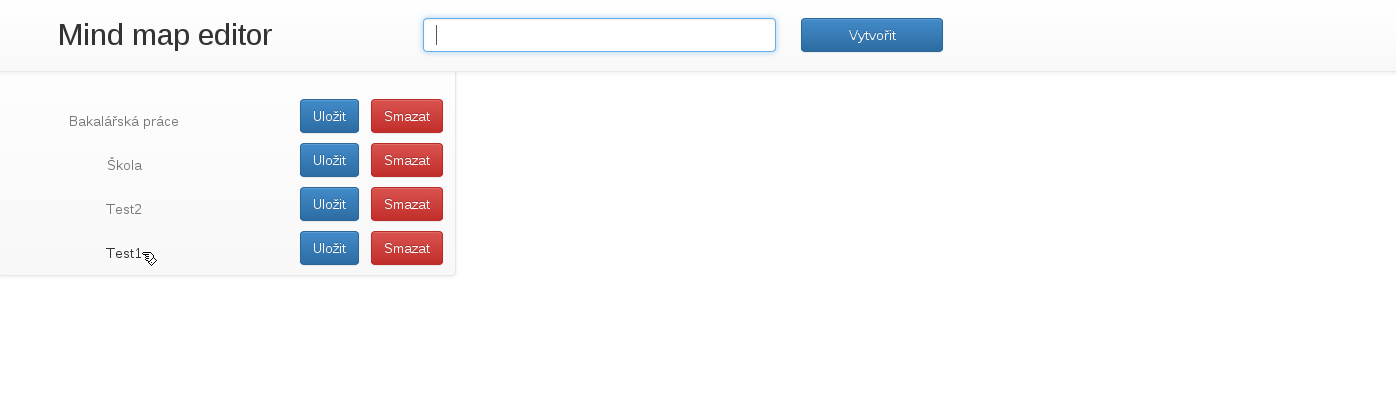
\includegraphics[width	=1\textwidth]{obrazky/mindmap1}
\par\end{centering}
\caption{Webová aplikace\label{fig:midnmap1}}
\end{figure}

\begin{figure}
\begin{centering}
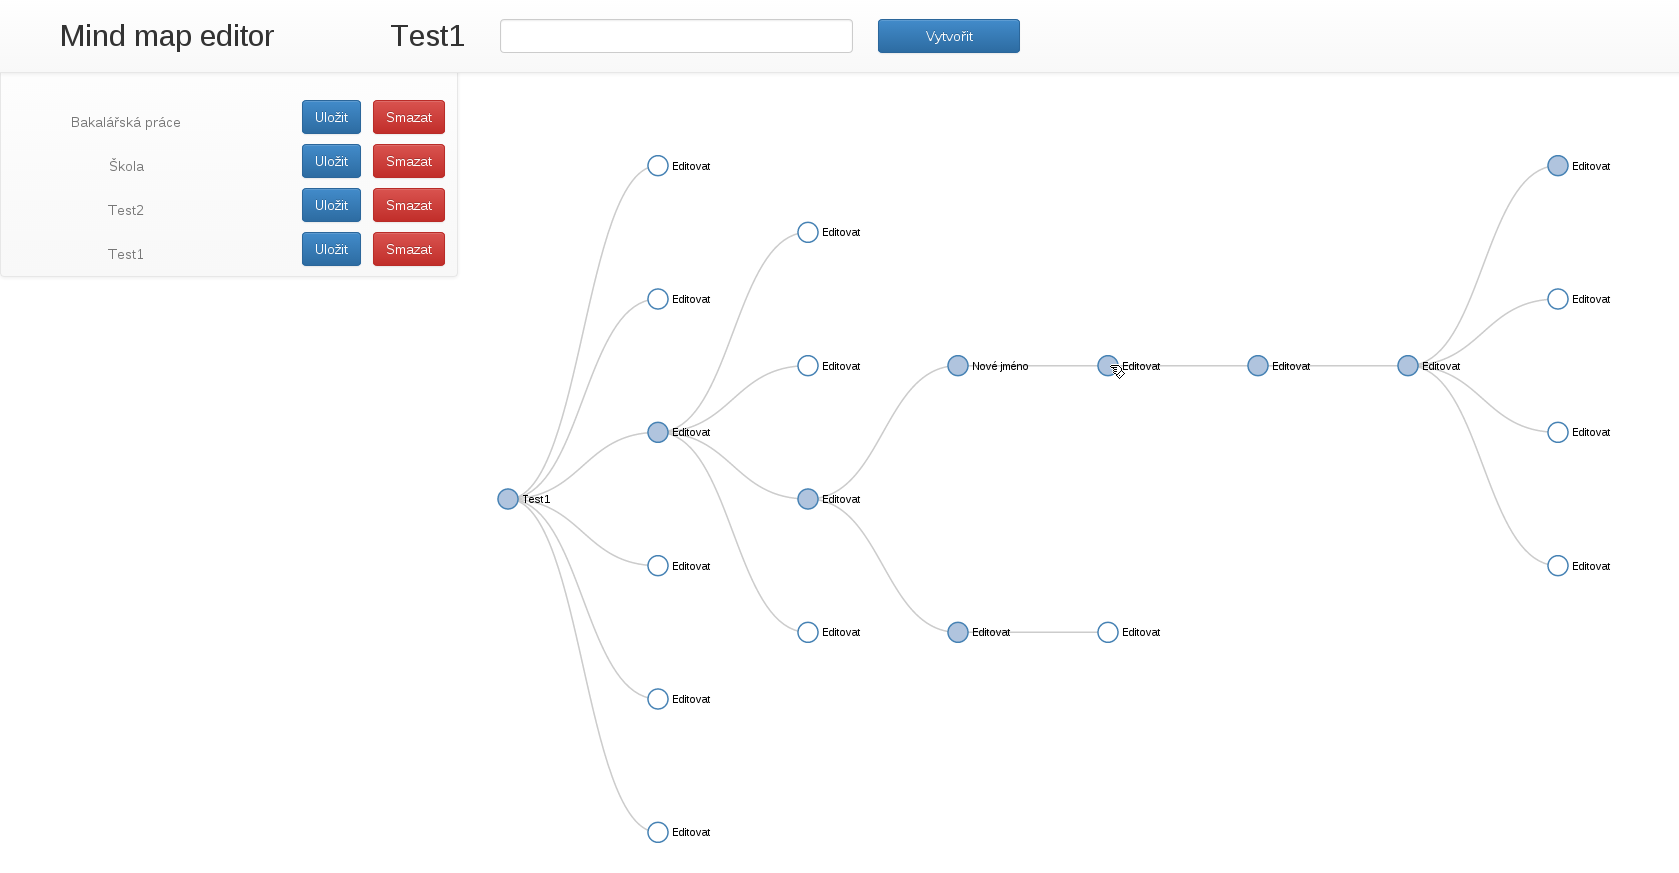
\includegraphics[width	=1\textwidth]{obrazky/mindmap2}
\par\end{centering}
\caption{Webová aplikace - otevření myšlenkové mapy\label{fig:midnmap2}}
\end{figure}

\begin{figure}
\begin{centering}
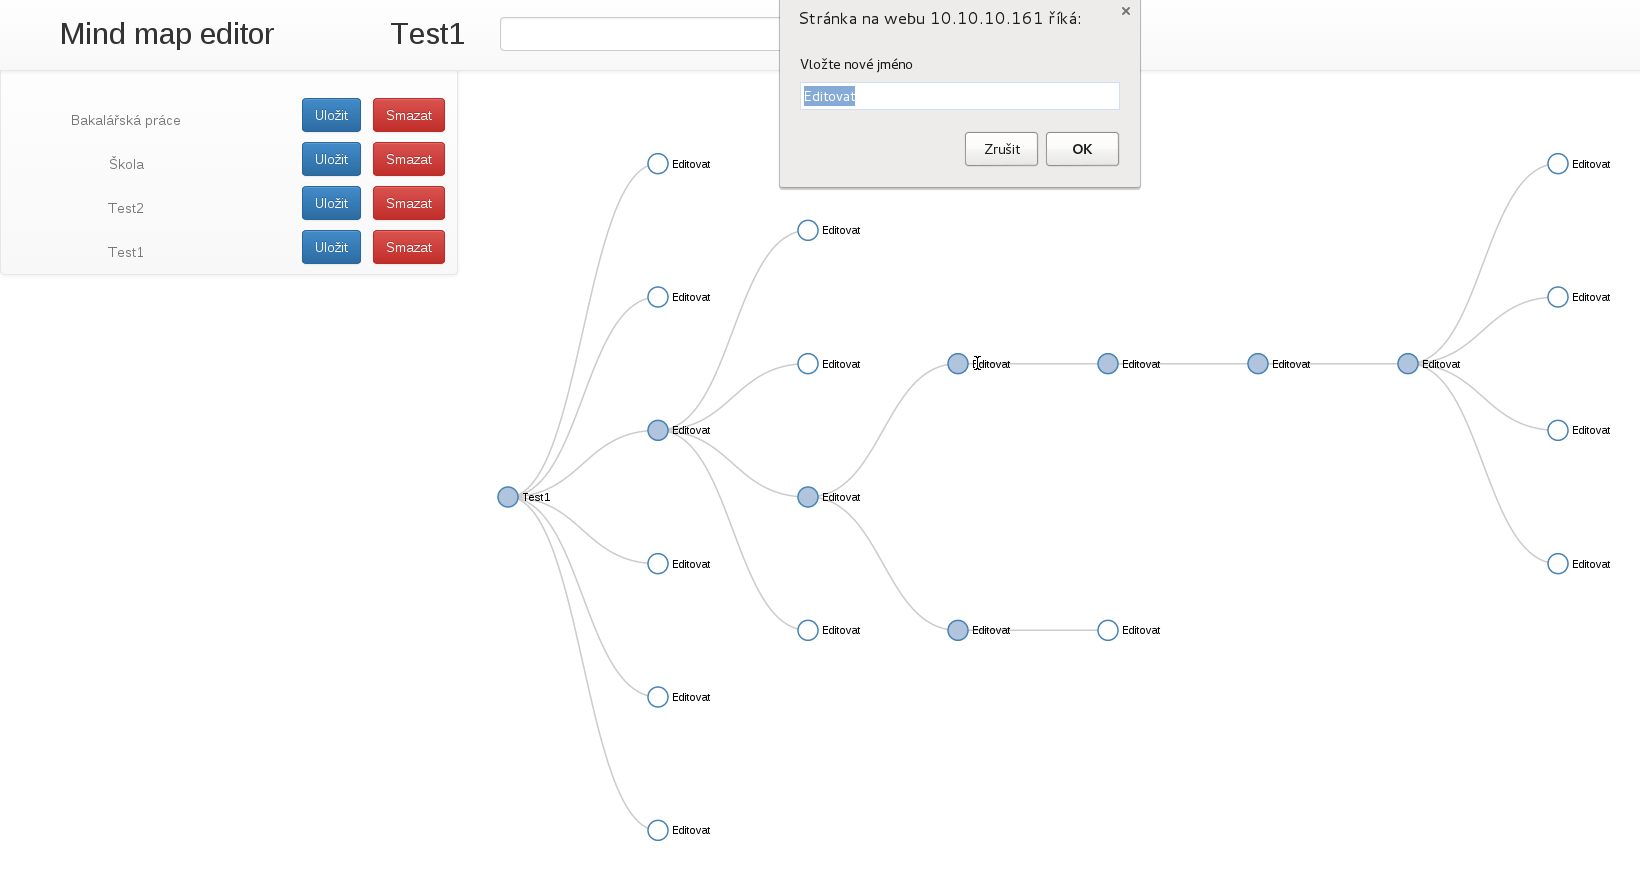
\includegraphics[width	=1\textwidth]{obrazky/mindmap3}
\par\end{centering}
\caption{Webová aplikace - akce - editace\label{fig:midnmap3}}
\end{figure}

\section{Základní software}

Jádrem serveru je operační systém Ubuntu\cite{ubuntu} 14.04 LTS\footnote{dlouhodobá podpora} Server Edition s kódovým označením 
Trusty Tahr. Je to osvědčený systém, který bude má zaručenou podporu do roku 2019. Systém má aplikaci pro správu softwarových balíků 
aptitude. Všechny aplikace kromě samotného Vert.x jdou hravě nainstalovat pře tento systém.

\subsection{Java}

Jako hlavní přísadou celého prostředí je otevřená implementace Java Platform, knihovna OpenJDK ve verzi 7.

\subsection{Vert.x}

Jediná služba, která se zatím nenachází jako systémový balíček je samotný Vert.x. Pro jeho instalaci je nutné stáhnout distribuci ze stránek platformy. Tento archiv potom rozbalit do požadované lokace. Následně stačí v závislosti na konkrétním systému přidat soubor \emph{vertx/bin/vertx} do systémové proměnné \emph{PATH}. Poté by měla být funkční interakce s platformou pomocí příkazové řádky. Příklad proměnné \emph{PATH} lze vidět v kapitole \ref{sub:service}. Správné nastavení lze otestovat napsáním \emph{vertx} do příkazové řádky. Správný výstup jsou pak pomocné informace pro komunikaci s platformou tzv. help.

\subsection{Databázový server}

Pro ukládání myšlenkových map je použita NoSQl databáze MongoDB ve verzi 2.6. MongoDB má za sebou více než pět let vývoje a několik obřích investic\cite{mongodb} do dalšího vývoje. V dnešní době existuje nespočet NoSQL databází, vzhledem k tomu, že již existuje Vert.x modul pro pohodlnou asynchronní spolupráci s touto databází, byla vybrána pravě tato NoSQL databáze. Pro instalaci stačí využít balíčkovací systém aptitude. Nastavení databáze lze ponechat ve výchozím stavu, kdy databáze naslouchá na portu 27017. Což lze vidět i z konfigurace aplikace v ukázce kódu \ref{confServ2}.

\begin{lstlisting}
apt-get install mongodb-server -y
\end{lstlisting}

\subsection{Nasazení produkční služby}\label{sub:service}

V současné verzi, (2.1.2) Vert.x nepodporuje běh v režimu daemon\footnote{je program, který běží v pozadí, čeká na události, které nastanou, reaguje na ně a poskytuje služby.}. Nasazení v režimu daemon je však nutnost pro běh v produkčním prostředí. Pro běh aplikace MindMap editoru byla využita systémová služba Supervisord\footnote{supervisord.org}, která běží jako linuxový daemon a stará se o běh aplikace, v případě pádu se ji pokusí znovu nasadit. Samotná konfigurace služby pro běh v Supervisordu pak obsahuje základní parametry. Ve verzi 3.0 je však plánovaná funkce běhu v režimu daemona a nebude tak tato berlička potřeba.

\begin{lstlisting}[caption=Konfigurace produkční služby]
[program:vertx_mindmap_editor]
directory=/srv/mindmap/app
environment=PATH="/srv/vert.x-2.1RC3/bin/vertx"
environment=JAVA_HOME="/usr/lib/jvm/java-7-openjdk-amd64/"
command=vertx runmod io.majklk~mindmapeditor~0.0.1 -conf /srv/mindmap/conf/allinone.json
user=root
autostart=true
autorestart=true
redirect_stderr=true
stdout_logfile=/srv/mindmap/app/app.log
stderr_logfile=/srv/mindmap/app/error.log
startsecs=10
stopwaitsecs=600
\end{lstlisting}

Nejdůležitější parametry jsou \emph{environment} a \emph{command}, které umožňují pohodlně spustit libovolnou aplikaci jako daemona.

\subsection{Interakce s Vert.x}\label{sub:interaction}

Díky modulu CrasHub Shell\footnote{https://github.com/crashub/mod-shell} se lze protokolem SSH\footnote{Secure Shell} přihlásit přímo do Vert.x. Modul pak nabízí možnost interakce s jednotlivými komponentami samotného Vert.x. Lze například posílat zprávy přes Event Bus nebo nasazovat nové moduly za běhu celé aplikace.
\begin{figure}[h]
\begin{centering}
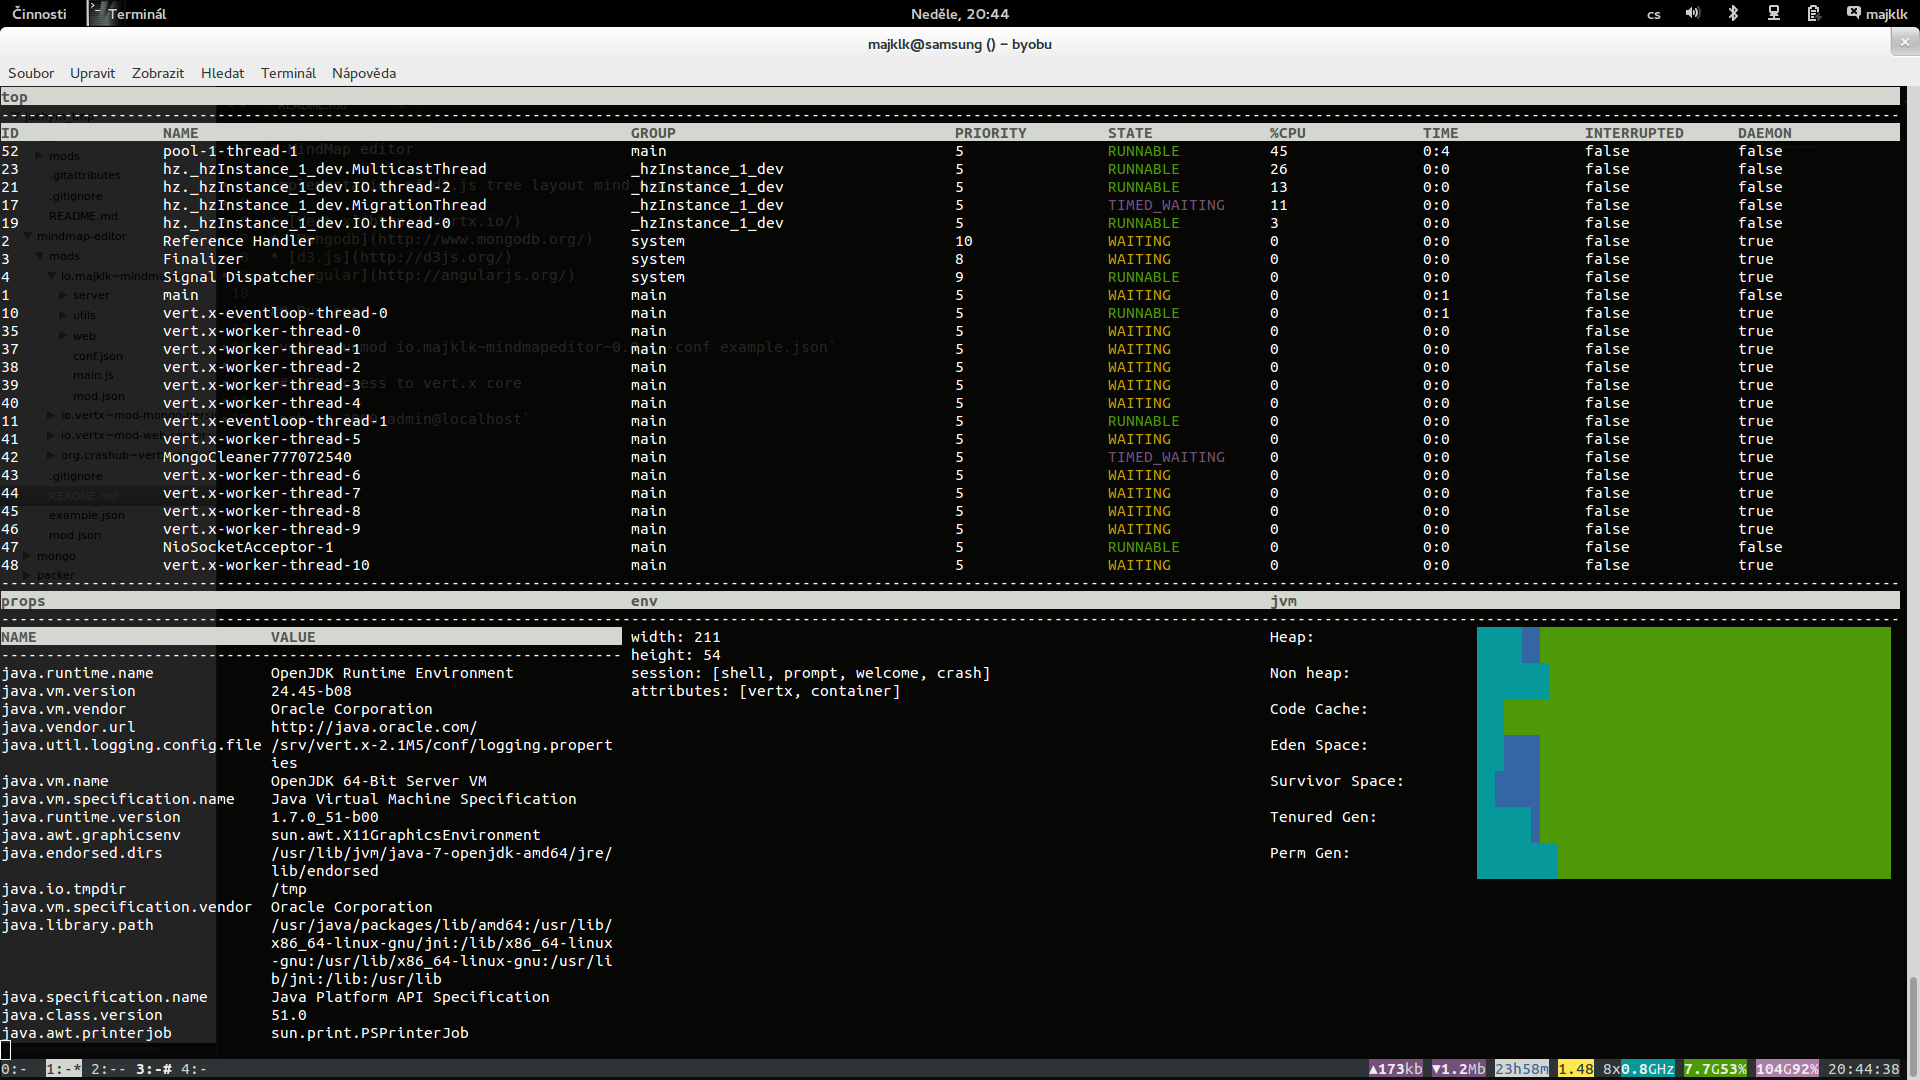
\includegraphics[scale=0.21]{obrazky/real_interaction}
\par\end{centering}
\caption{Modul CrasHub Shell\label{fig:real_interaction}}
\end{figure}

Pro nasazení modulu stačí přidání klíče \emph{shell} do konfigurace server 2. Po nasazení aplikace začne tento server poslouchat na portu 2000.

\begin{lstlisting}[caption={Konfigurace modulu CrasHub Shell},label=confServ2]
{
    "name": "MindMap editor server 2 databázový modul, obrazkový exporter",
    "shell": {
      "crash.auth": "simple",
      "crash.auth.simple.username": "admin",
      "crash.auth.simple.password": "heslo",
      "crash.ssh.port": 2000
    }
}
\end{lstlisting}

Samotný modul nabízí nepřeberné množství možností jak spravovat aplikace nebo ji naživo škálovat. Lze také jednoduše přidat vlastní příkazy a rozšířit tak možnosti tohoto modulu. Na obrázku \ref{fig:real_interaction} je hlavní přehledová stránka, na které lze vidět činnost vytížení a status všech vláken v celém clusteru. Dostupné jsou také informace o velikosti zásobníku, paměti či verze Javy. 

\section{Škálování}\label{sub:Scaling}

Škálování je nedílnou součástí životního cyklu aplikace. Ne zřídka dojde aplikace do situace, kdy začne být pomalá či často padat pod velkým náporem klientů. V následující kapitole proto rozebírám možnosti škálování Vert.x aplikací.

\FloatBarrier

\subsection{Vertikální}

Samotné vertikální škálování lze efektivně řešit až na aplikační úrovni. Jak již bylo zmíněno v kapitole \ref{sub:multireactor} voláním \emph{Runtime.getRuntime().availableProcessors()}, lze získat počet procesorových jader a s tím dále pracovat. Upravením předchozích příkazů však docílíme shodného výsledku.

\begin{lstlisting}
command=vertx runmod io.majklk~mindmapeditor~0.0.1 -instances 4 -conf
\end{lstlisting}

\subsection{Horizontální}\label{sub:praktCluster}

Dle návrhu architektury na obrázku \ref{fig:architecture_real} bude aplikace nasazena na dva servery. První bude naslouchat na port 80 a poběží zde Webový server(HTTP Server). Tento server má vnitřní IP adresu \emph{10.10.10.161}. Druhé rozhraní má připojené do internetu. Na druhém serveru je část aplikace, která komunikuje s databází a modul pro vzdálenou interakci s Vert.x. Jeho IP adresa je \emph{10.10.10.162}. Pro propojení obou instancí je potřeba upravit spouštěcí příkaz v konfiguraci Supervisoru.

\begin{lstlisting}[caption=Spuštění clusteru na Serveru 1]
command=vertx runmod io.majklk~mindmapeditor~0.0.1 -conf /srv/mindmap/conf/webserver.json -cluster -cluster-host 10.10.10.161
\end{lstlisting}

\begin{lstlisting}[caption=Spuštění clusteru na Serveru 2]
command=vertx runmod io.majklk~mindmapeditor~0.0.1 -conf /srv/mindmap/conf/dbserver.json -cluster -cluster-host 10.10.10.162
\end{lstlisting}

\subsection{Ladění výkonnosti}\label{sub:performenceScale}

Hlavní sada vláken, tedy event loopů je ve výchozím nastavení na hodnotě odpovídající volání funkce \emph{Runtime.getRuntime().availableProcessors()}. Tuto hodnotu lze změnit nastavením systémové proměnné \emph{vertx.pool.eventloop.size}. Nastavením \emph{vertx.pool.worker.size} pak lze změnit velikost poolu pro dlouhotrvající operace, která je ve výchozím nastavení na hodnotě 20.

\section{Vysoká dostupnost}

Pro zajištění vysoké dostupnosti klíčových prvků aplikace, je potřeba upravit architekturu clusteru. Před webový server je postaven load balancer\footnote{služba zajištující vyrovnávání zatížení} v tomto případě HA proxy, která při úpadku jednoho z webových serverů přesměruje komunikaci na server druhý. Vert.x cluster je rozdělený na dvě HA skupiny (obr.\ref{fig:architecture_ideal}), které se liší svým zaměřením. První dva servery slouží jako webové a jsou napojeny na HA proxy. Další dva slouží pro komunikaci s databází, která na nich, přímo běžet nemusí. V této HA skupině je dále modul pro interakci s Vert.x. Díky specifikaci HA skupiny nikdy nedojde k nasazení modulu na webovém serveru a tedy otevření SSH na portu 2000.

\begin{lstlisting}[caption=Vysoká dostupnost na databázovém serveru 2]
command=vertx runmod io.majklk~mindmapeditor~0.0.1 -conf /srv/mindmap/conf/dbserver.json -cluster-host 10.10.10.162 -ha -hagroup skupina-1
\end{lstlisting}

Když je specifikován parametr \emph{-ha}, lze automaticky vypustit parametr \emph{-cluster}.

\begin{figure}
\begin{centering}
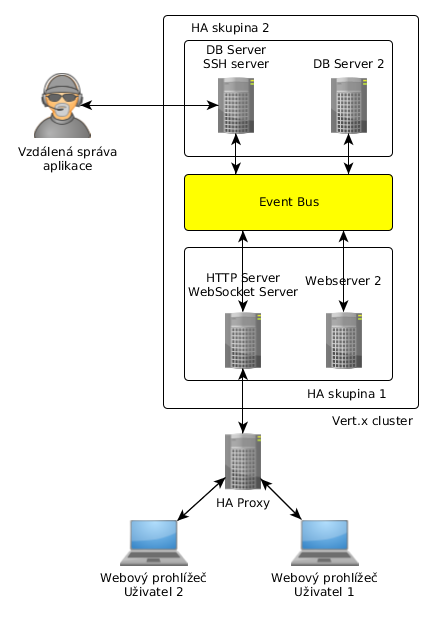
\includegraphics[scale=0.5]{obrazky/architecture_ideal}
\par\end{centering}
\caption{Ideální architekutra nasazení aplikace\label{fig:architecture_ideal}}
\end{figure}

\section{Integrace do stávájící Java aplikace}

Pokud je to jakkoliv jen možné, je vhodné se integraci vyhnout. Pokud však nejde jinak, existují dvě varianty jak integrovat platformu:

\begin{enumerate}
\item PlatformManager
\item Pomocí jar souboru
\end{enumerate}

\begin{lstlisting}[caption=Integrace do stávající Java aplikace]

//díky platform managerovi lze provádět stejné úkony jako v příkazové řádce
PlatformManager pm = null;
pm = PlatformLocator.factory.createPlatformManager();

JsonObject conf = new JsonObject().putString("foo", "wibble");

pm.deployModule("com.mycompany~my-module~1.0", conf, 10, new AsyncResultHandler<String>() {
    public void handle(AsyncResult<String> asyncResult) {
        if (asyncResult.succeeded()) {
            System.out.println("Deployment ID is " + asyncResult.result());
        } else {
            asyncResult.cause().printStackTrace();
        }
    }
});
\end{lstlisting}

V takovém případě bude platforma hledat \emph{cluster.xml} a \emph{repos.txt} v proměnné classpath.


\chapter[Závěr ]{Dobrá rada na závěr}

\LyX{} je vynikající editor, který vám usnadní napsání rozsáhlejší
práce typu bakalářka nebo diplomka. Editor si hravě poradí s komplikovanými
úlohami jako je vkládání křížových odkazů, vytvoření seznamu literatury
a citování literatury v textu, vytvoření obsahu a rejstříku. Bez většího
úsilí bude vaše práce  typograficky na úrovni.

Používáte-li %
\marginpar{\textbf{\Huge !}%
}\LyX{} jen na psaní bakalářky, \emph{nesnažte se} naučit vše, co umí!
Zabralo by to více času než celá bakalářka! Naučte se jen pár nezbytností
a pište a pište a pište! Až budete mít dopsán a zkontrolován text,
můžete si pohrát s výběrem vzhledu vhodného pro vaši práci, s výběrem
písma, typu záhlaví stránek, hlaviček kapitol atd. Teprve nakonec
udělejte závěrečnou typografickou revizi textu. Zejména zkontrolujte
polohu plovoucích objektů (případně je přemístěte na vhodnější místo)
a odstraňte vdovy a sirotky (osamělé řádky)%
\footnote{Nejsnáze odstranit tak, že z textu vypustíte (nebo do něj přidáte)
pár slov či vět anebo úpravou odstavců.%
}.


\begin{thebibliography}{10}

\bibitem{whoControlVertx}Phipps, Simon \emph{Who controls Vert.x: Red Hat, VMware, or neither?}
{[}online]. {[}cit. 2014-06-30]. Dostupný z WWW: \url{http://www.infoworld.com/d/open-source-software/who-controls-vertx-red-hat-vmware-or-neither-210549}

\bibitem{JAX}Kamali, Masoud \emph{The Winners of the JAX Innovation Awards 2014}
{[}online]. {[}cit. 2014-06-30]. Dostupný z WWW: \url{http://jax.de/awards2014/}

\bibitem{serialTest}Gardoh, Ed \emph{Parallel Processing and Multi-Core Utilization with Java}
{[}online]. {[}cit. 2014-03-22]. Dostupný z WWW: \url{http://embarcaderos.net/2011/01/23/parallel-processing-and-multi-core-utilization-with-java/}

\bibitem{reactorPattern}Merta, Zdeněk\emph{Vert.x jOpenSpace 2013} {[}online].
{[}cit. 2014-03-22]. Dostupný z WWW: \url{http://jopenspace.cz/2013/presentations/zdenek-merta-vert.x.pdf}

\bibitem{forkJoin}Ponge, Julien \emph{ Fork and Join: Java Can Excel at Painless Parallel Programming Too! } {[}online].
{[}cit. 2014-03-22]. Dostupný z WWW: \url{http://www.oracle.com/technetwork/articles/java/fork-join-422606.html}

\bibitem{javaChangelog}\emph{ Package java.util.concurrent Description} {[}online].
{[}cit. 2014-03-22]. Dostupný z WWW: \url{http://docs.oracle.com/javase/7/docs/api/java/util/concurrent/package-summary.html#package_description}

\bibitem{inMemoryDataGrid}Sun Song, Ki \emph{ Understanding Vert.x Architecture - Part II } {[}online].
{[}cit. 2014-03-22]. Dostupný z WWW: \url{http://www.cubrid.org/blog/dev-platform/introduction-to-in-memory-data-grid-main-features/}

\bibitem{vertxArchitectureDiagram}Jaehong, Kim\emph{ Introduction to In-Memory Data Grid: Main Features } {[}online].
{[}cit. 2014-03-22]. Dostupný z WWW: \url{http://www.cubrid.org/blog/dev-platform/understanding-vertx-architecture-part-2/}

\bibitem{javaProgramovani}Pitner, Tomáš\emph{ Programování v jazyce Java } {[}online].
{[}cit. 2014-03-22]. Dostupný z WWW: \url{http://www.fi.muni.cz/~tomp/slides/pb162/printable.html}

\bibitem{vlaknaCvut}Lažanský, J.\emph{ Procesy a vlákna } {[}online].
{[}cit. 2014-03-22]. Dostupný z WWW: \url{http://labe.felk.cvut.cz/vyuka/A4B33OSS/Tema-03-ProcesyVlakna.pdf}

\bibitem{eventLoops}Fox, Tim\emph{ Event loops } {[}online].
{[}cit. 2014-03-22]. Dostupný z WWW: \url{http://vertx.io/manual.html#event-loops}

\bibitem{session}Kosek, Jiří\emph{ Session proměnné } {[}online].
{[}cit. 2014-03-22]. Dostupný z WWW: \url{http://www.kosek.cz/clanky/php4/session.html}

\bibitem{mq}Janssen, Cory\emph{ Message Queue } {[}online].
{[}cit. 2014-03-22]. Dostupný z WWW: \url{http://www.techopedia.com/definition/25971/message-queue}

\bibitem{benchmark}Froemke, Dina\emph{ Framework Benchmarks Round 8 } {[}online].
{[}cit. 2014-03-22]. Dostupný z WWW: \url{http://www.techempower.com/blog/2013/12/17/framework-benchmarks-round-8/}

\bibitem{benchmarkTim}Fox, Tim\emph{ Vert.x vs node.js simple HTTP benchmarks } {[}online].
{[}cit. 2014-03-22]. Dostupný z WWW: \url{http://vertxproject.wordpress.com/2012/05/09/vert-x-vs-node-js-simple-http-benchmarks/}

\bibitem{scaling}Osuszek, Lukasz\emph{ Distributed Architecture of Enterprise Information Systems } {[}online].
{[}cit. 2014-07-31]. Dostupný z WWW \url{http://www.soainstitute.org/resources/articles/distributed-architecture-enterprise-information-systems}

\bibitem{d3js}Bostock, Mike\emph{ Collapsible Tree } {[}online].
{[}cit. 2014-07-31]. Dostupný z WWW \url{http://bl.ocks.org/mbostock/4339083}

\bibitem{ubuntu}Canonical Ltd.\emph{ Ubuntu Server Edition } {[}online].
{[}cit. 2014-08-01]. Dostupný z WWW \url{http://www.ubuntu.com/server}




\end{thebibliography}

\addcontentsline{toc}{chapter}{Literatura} 

\cleardoublepage{}

\appendix
\pagenumbering{Roman}\addcontentsline{toc}{part}{Přílohy}\thispagestyle{empty}  \renewcommand{\appendixname}{P\v{r}iloha}%%přílohy, číslování římskými


\part*{Přílohy}

\listoffigures

\listoftables

\listoflistings


\end{document}
